\section{Analysis strategy}\label{sec:AnalysisStrategy}

\subsection{Introduction}
The analysis strategy for the high mass search with 2016 data in the
$\mathrm{W^+W^-}\to2\ell2\nu$ decay channel  is similar to the previous high
mass analysis with 2015 data~\cite{CMS-PAS-HIG-16-023}, but has several improvements. \\
In the opposite-flavour $\mathrm{W^+W^-}\to e^{\pm} \mu^{\mp} 2\nu$ final
state four different jets-categories are defined (they were three in
~\cite{CMS-PAS-HIG-16-023}): 0-jet, 1-jet, 2-jet-non VBF and VBF. The 2 jet
non-VBF category is new with respect to ~\cite{CMS-PAS-HIG-16-023}.
A same-flavour (SF) $\mathrm{W^+W^-}\to e^+ e^- 2\nu$ and $\mathrm{W^+W^-}\to
\mu^+ \mu^- 2\nu$ category, has been added in the VBF phase space. Indeed, the VBF
selection cuts are sufficiently tight to reduce the otherwise overwhelming
Z+jets background to a manageable level.

Whenever we count jets in this analysis we always refer to AK4 jets with $\pt>30$\GeV.

Events are requested to pass single or double lepton triggers. Leptons should have a mini-
mum $p_T$ of 10 (13) GeV for the muon (electron) candidate. One of the two leptons should also
have a $p_T$ greater than 25 GeV and two leptons are requested to be well identified and isolated,
to reject non-prompt leptons and leptons coming from QCD sources. These selections are in
common to all phase spaces, and are detailed in~\cite{AN-17-082}.


The main production mode for the Higgs boson production over the all mass spectrum is the gluon-gluon fusion process (ggH). At a center-of-mass energy of 13\TeV the ggH cross section for a Higgs boson mass ($m_\mathrm{H}$) of 125\GeV is 43.92\,pb~\cite{temphiggsxsecs}, that is almost one order of magnitude larger than the second process  in terms of cross section at that mass, VBF, with 3.748\,pb~\cite{temphiggsxsecs}. The ggH cross section decreases with $m_\mathrm{H}$ but the VBF/ggH cross section ratio increases with the mass, making the VBF production mechanism more and more important as $m_\mathrm{H}$ approaches to high values.\\
The signal samples are interpreted in terms of the EWK singlet model described
in Sec~\ref{sec:signalModel} below. The Higgs boson width and lineshape is reweighted at generator level according to the parameters defined in the model.
The interference effects between the ggH signal, the ggWW background and SM
Higgs boson, that are expected to slightly change the lineshape of the signal
distribution, have been fully taken into account, as detailed in
Sec.~\ref{sec:interference}. The interference between the $\mathrm{W^+W^-}\to2\ell2\nu$ and $\mathrm{ZZ}\to2\ell2\nu$ is negligible due to the different phase space characteristic of these processes. 

\subsection{Discriminating variable}
The analysis presented in this note is a shape analysis, meaning that after
applying selection cuts detailed in Secs~.\ref{sec:OF} and \ref{sec:SF} below,
we do not simply count events, but rather we fit a data histogram of a
discriminating variable with the sum of signal and background templates, and
extract the signal yield from the fit.
The variable with the best discriminating value would be the invariant mass of
the four lepton, which is not possible to reconstruct in the \WW channel due
to neutrinos.
%The branching fraction from Higgs to a \WW pair is the largest for mass values above 200\GeV~\cite{Heinemeyer:2013tqa}, and the $\mathrm{W^+W^-}\to2\ell2\nu$ decay channel is the second in terms of branching ratio, surpassed only by the semi-leptonic decay mode. 
%In addition  the leptonic decay chosen boasts a very clear experimental signature,  and though there are several backgrounds affecting the final state,  
%there are some kinematic variables that can be used to separate the signal, leading to a good and clearn signal sensitivity.

In the SM Higgs,  a shape analysis based on two-dimensional templates of $m_{\ell \ell}$ versus $m_T^H$ in each of the categories is performed, where  the transverse mass  $m_T^H$ variable is defined as  
\begin{equation}
 m_T^H = \sqrt{2p_{\rm T}^{\ell\ell}\MET(1-\mathrm{cos}\Delta\phi(\ell\ell, \ptvecmiss))}
\end{equation}
where $\Delta\phi(\ell\ell, \ptvecmiss)$ is the azimuthal angle between the dilepton momentum and \ptvecmiss.\\
However  $m_T^H$ (and also $m_{\ell \ell}$) is not very sensitive to the
signal mass hypothesis, so a \textit{new} variable $m_T^I$ defined as the visible mass,
\begin{equation}
 m_T^I = \sqrt{ (p_\mathrm{\ell\ell} + \MET)^2 - (\vec{p}_\mathrm{\ell\ell} + \ptvecmiss)^2 }
\end{equation}
has been introduced in 2015 analysis to discriminate better the signals generate at different masses.
The distribution of the variables defined above are shown in
Fig.~\ref{fig:mt_nocuts}, where the better power of $m_T^I$ in discriminating
different mass hypotheses over other variable is visible.

\begin{figure}[htbp]
\centering
\subfigure[True generated mass]{
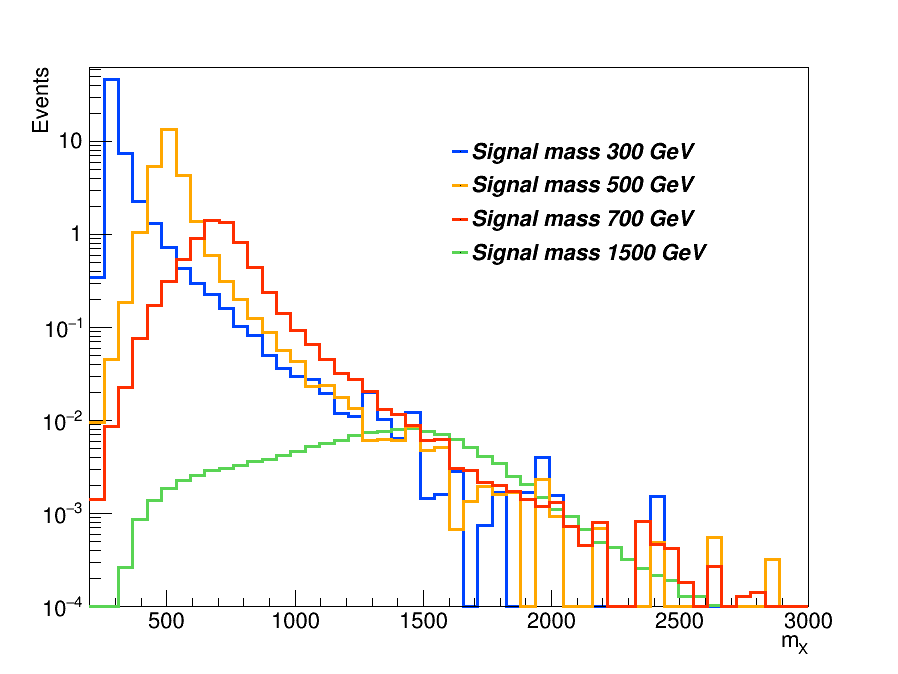
\includegraphics[width=0.45\textwidth]{Figs/Distribution_higgsLHEmass_cuts_nocuts.png}
}
\subfigure[$m_T^H$]{
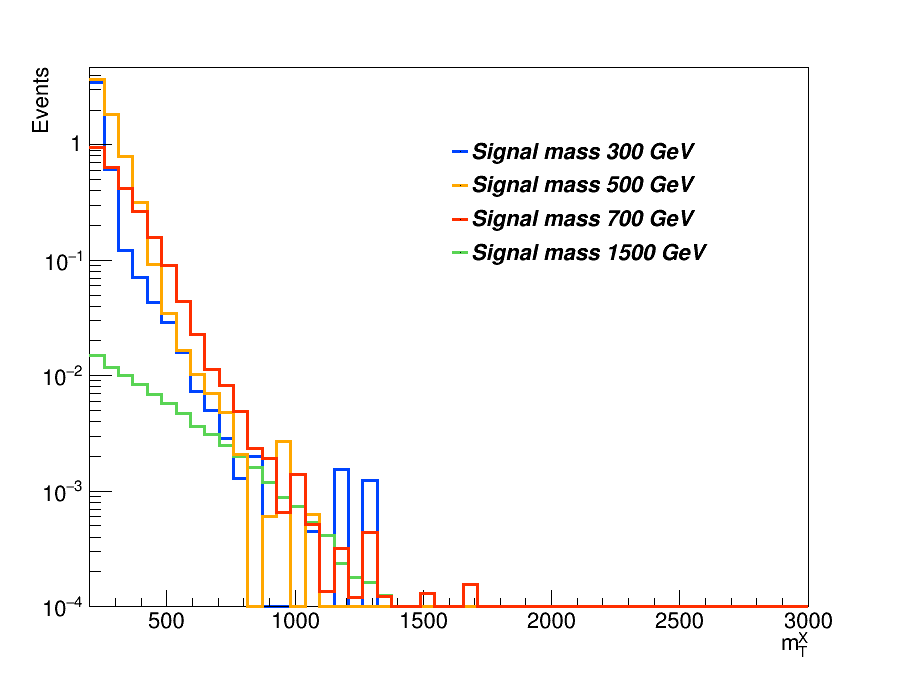
\includegraphics[width=0.45\textwidth]{Figs/Distribution_mth_cuts_nocuts.png}
}
\\
\subfigure[$m_{\ell \ell}$]{
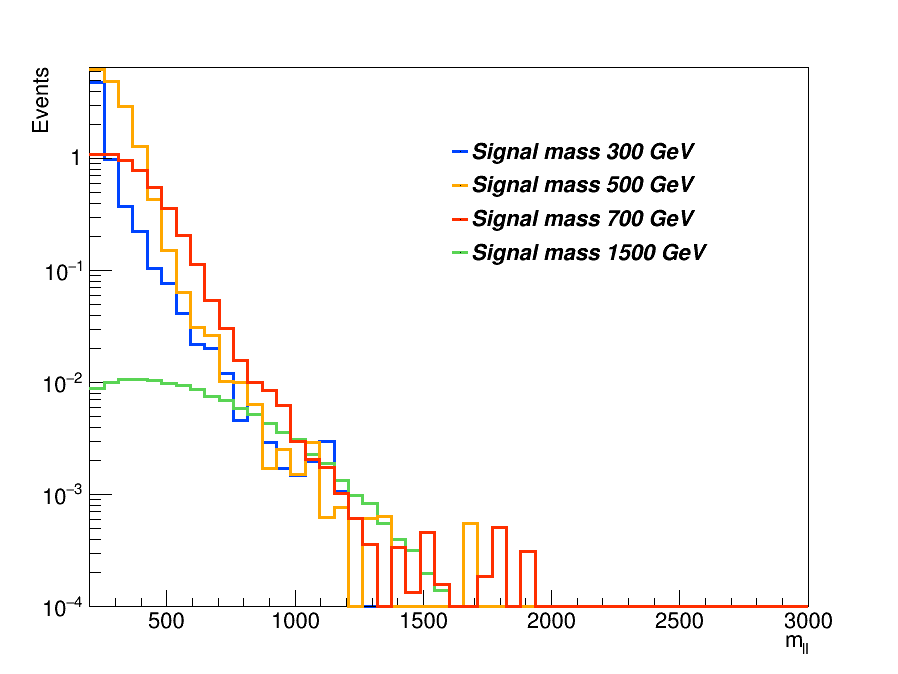
\includegraphics[width=0.45\textwidth]{Figs/Distribution_mll_cuts_nocuts.png}
}
\subfigure[$m_T^I$]{
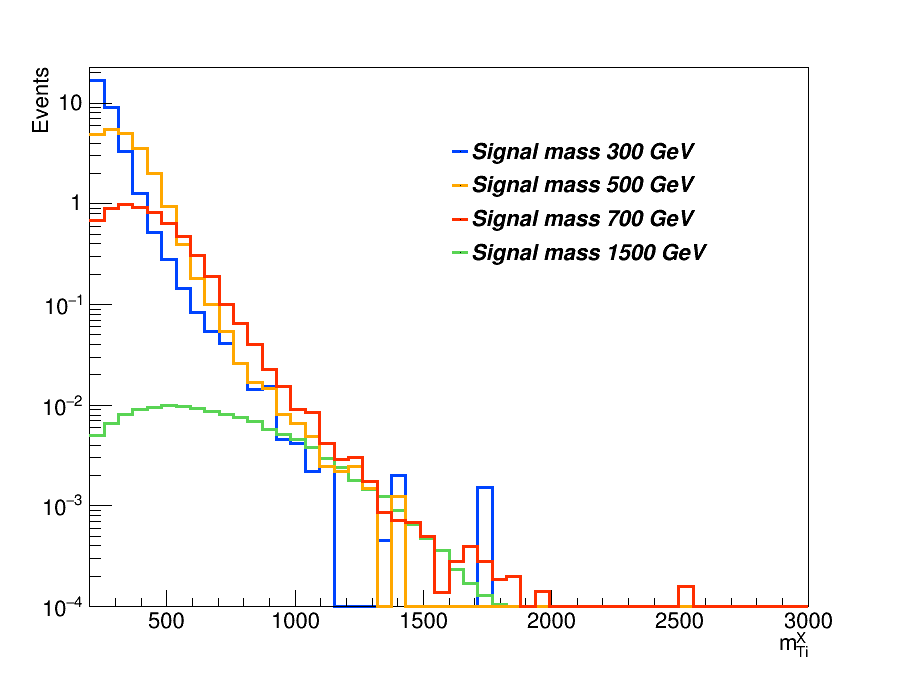
\includegraphics[width=0.45\textwidth]{Figs/Distribution_mTi_cuts_nocuts.png}
}
\caption{
    Distributions of the generated mass, $m_T^H$, $m_{\ell \ell}$ and  $m_T^I$
    variables for different Higgs mass hypothesis, without
    any selection. The same distribution after the OF selection are shown in Appendix \ref{sec:AppA}.}
    \label{fig:mt_nocuts}
\end{figure}



\subsection{Signal interpretation}
\label{sec:signalModel}

The signal is interpreted in terms of the electroweak singlet model, representing a scalar mixing with the 125\GeV Higgs boson. This model relies on two parameters: the scale factor of the couplings of the high mass resonance with respect to the SM, $C'$, and the branching fraction of the electroweak singlet to non-SM decays modes, $BR_\mathrm{new}$. The electroweak singlet signal strength, $\mu'$ and the modified width, $\Gamma'$, are related with the parameters in the model by the following equations:

\begin{equation}
\mu' = C'^2 \cdot (1 - BR_\mathrm{new})
\end{equation}
\begin{equation}
\Gamma' = \Gamma_\mathrm{SM} \cdot \frac{C'^2}{1 - BR_\mathrm{new}}
\end{equation}

The available Higgs signal samples for different mass hypothesis have been reweighted according to this model. At the moment only the $BR_\mathrm{new} = 0$ hypothesis has been investigated while we tested different $C'$ values.
In Fig.~\ref{fig:cprime} are shown the \mll and \mt templates corresponding to a Higgs boson mass of 700\GeV for three different $C'$ values: $C' = 1$, corresponding to the SM Higgs decay width, $C'=0.5$, corresponding to $\Gamma' = 2.5\cdot10^{-2}\,\Gamma_\mathrm{SM}$, and $C'=0.1$, corresponding to $\Gamma' = 10^{-2}\,\Gamma_\mathrm{SM}$. A value of $BR_\mathrm{new} = 0$ is considered in all cases. We note that the signal shape is not very sensitive to different $C'$ values.

\begin{figure}[htbp]
\centering
\subfigure[Simulated LHE signals]{
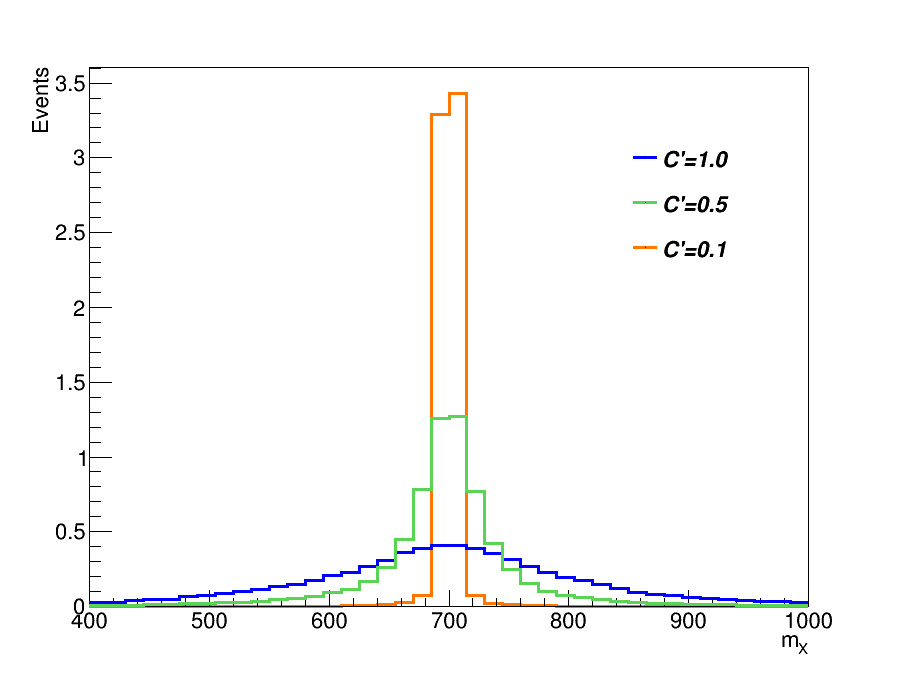
\includegraphics[width=0.45\textwidth]{Figs/higgsLHEmass700_cuts_nocuts.png}
}
\subfigure[$m_T^H$]{
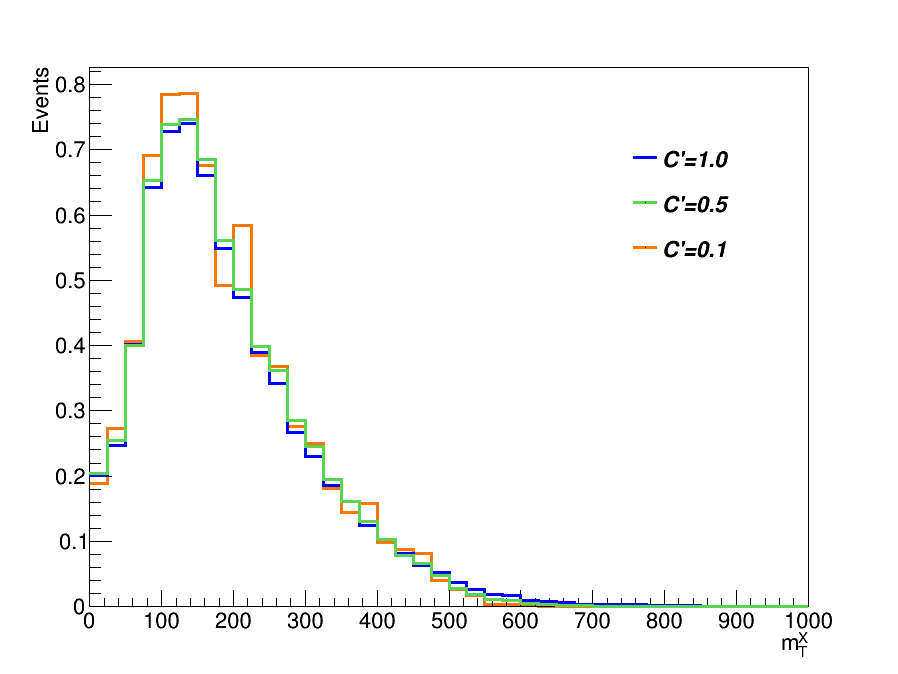
\includegraphics[width=0.45\textwidth]{Figs/mth700_cuts_nocuts.png}
}
\\
\subfigure[$m_{\ell \ell}$]{
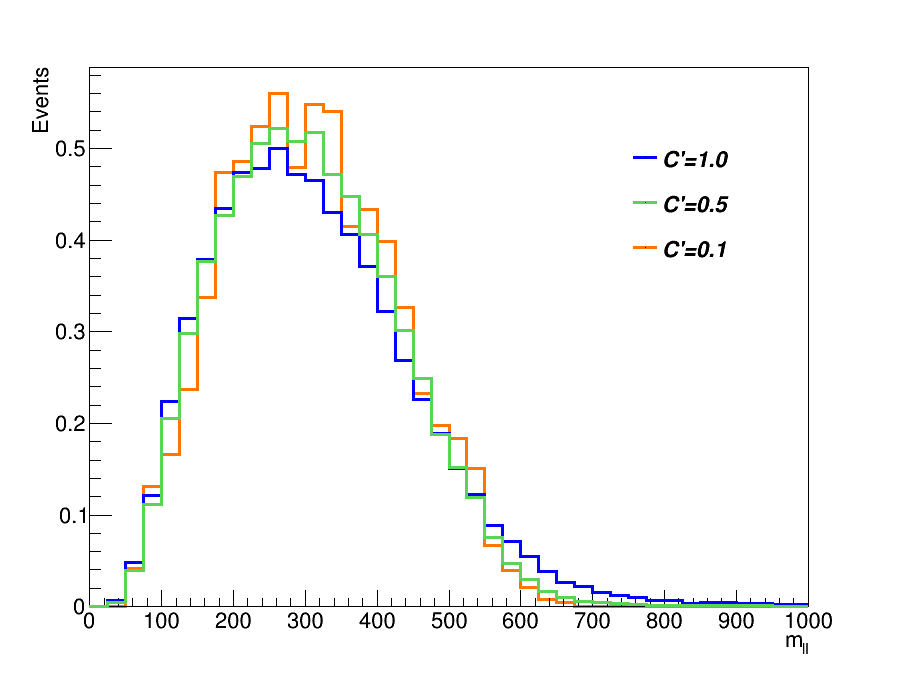
\includegraphics[width=0.45\textwidth]{Figs/mll700_cuts_nocuts.png}
}
\subfigure[$m_T^I$]{
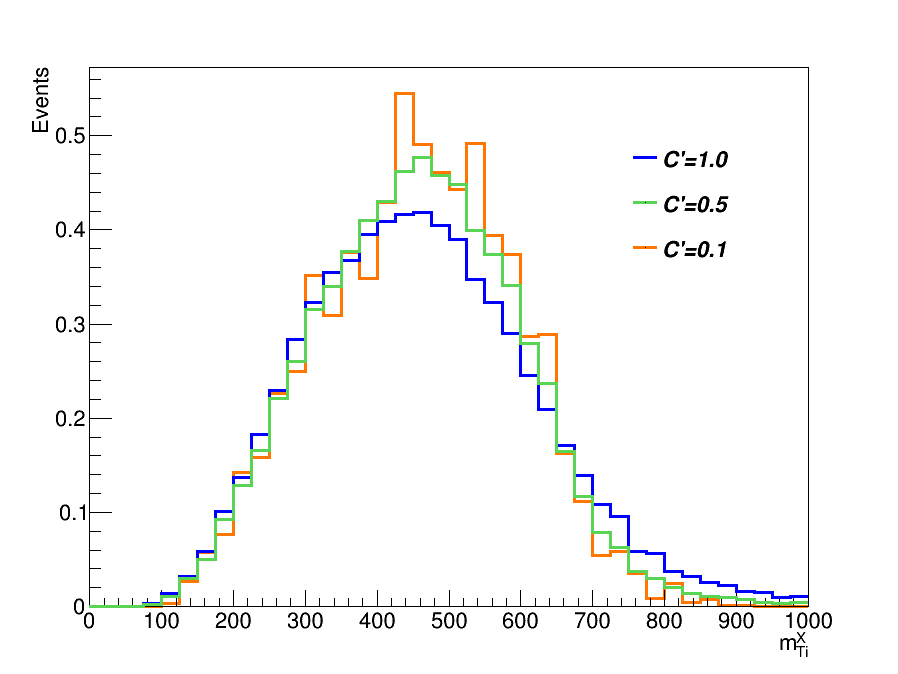
\includegraphics[width=0.45\textwidth]{Figs/mTi700_cuts_nocuts.png}
}
\caption{ 
    Distributions of the LHE-signals, $m_T^H$, $m_{\ell \ell}$ and  $m_T^I$ variables at generator level for different values of $C'$, without any selection. The same distribution after the OF selection defined in Section XX cuts are shonw in Appendix \ref{sec:AppB}.}
    \label{fig:cprime}
\end{figure}



\subsection{Study of the interference effects: ggH case}
\label{sec:interference}

When a resonance with a non negligible width is considered, it is important to take into account also the interference effects both with the background and the H(125) off-shell tail.
In this analysis  we take into account the interference effects between the
new signal X produced in gluon fusion, the ggWW continuum and the off-shell
H(125) tail. This is achieved in the MCFM+JHUGen framework, including NNLO
corrections for cross section using HNNLO program based on MCFM, in exactly
the same fashion this is achieved in ZZ high mass searches.
The MELA package is used to reweight the signal processes generated with \textsc{Powheg}+\textsc{JHUGen} in order to obtain the interference terms between X, the gg$\to$WW background and the H(125) off-shell tail.
The effect of the various interference terms are shown in ~\ref{fig:X300} for
the $M_\mathrm{X}$ variable at generator level. The contribution of the interference of X with gg$\to$WW and with H(125) have opposite sign and partially cancel out. This cancellation effect is different for different resonance masses.
The interference contribution is thus non negligible and is included in the
fit. \\
To prevent possible negative probability distribution function of the interference,  during the fit the signal yield is computated as [],
\begin{equation}
Yield=\sqrt{\mu} \times (S+B+I)+ (\mu -\sqrt{\mu}) \times (S) + (1-\sqrt{\mu}) \times (B)
\end{equation}
where  $S$ is the signal, $B$ the background and I the interference
%In particular during the fit the interference term is scaled by the square root of the signal strength.

The effect of all the interference terms on the $m_T^H$, $m_{\ell \ell}$ and $m_T^I$ variables for different cuts (0-jet, 1-jet, 2-jets and VBF, for cuts definition see Sec. 5) and different mass points  are shown in Fig.\ref{fig:300}, Fig.\ref{fig:700} and Fig.\ref{fig:1500}.


\begin{figure}[htbp]
\centering
\subfigure[mass 300 GeV]{
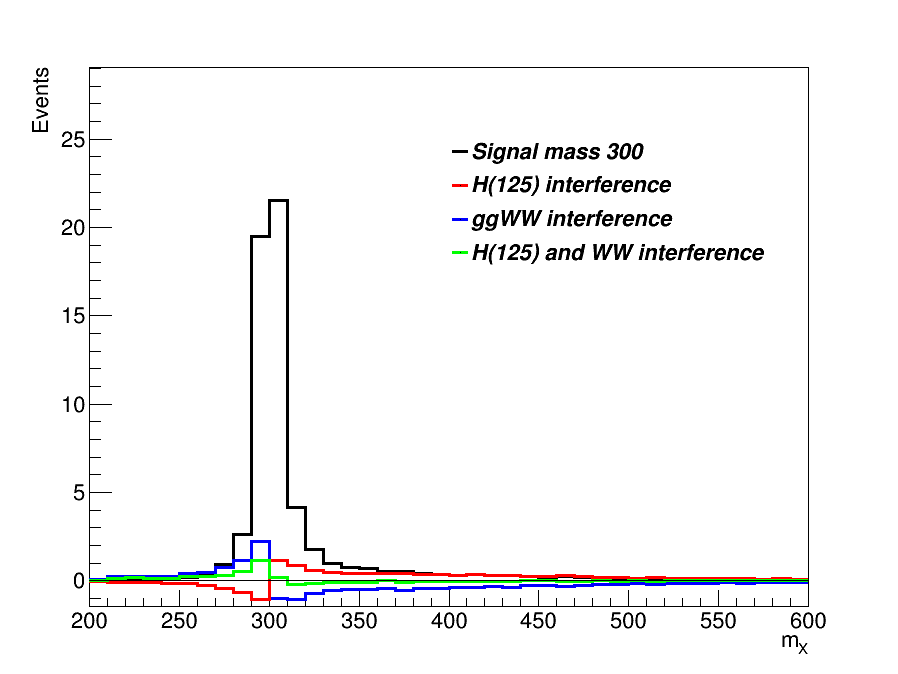
\includegraphics[width=0.45\textwidth]{Figs/Interference_higgsLHEmass300_cuts_nocuts.png}
}
\subfigure[mass 400 \GeV. Log scale]{
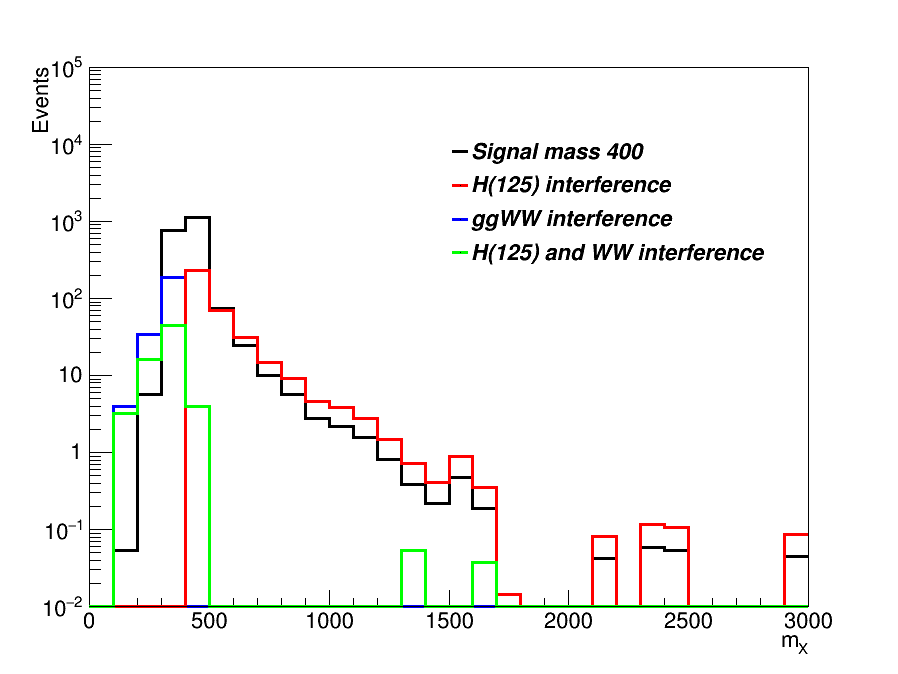
\includegraphics[width=0.45\textwidth]{Figs/Interference_higgsLHEmass400_cuts_nocuts.png}
}
\\
\subfigure[mass 700 \GeV]{
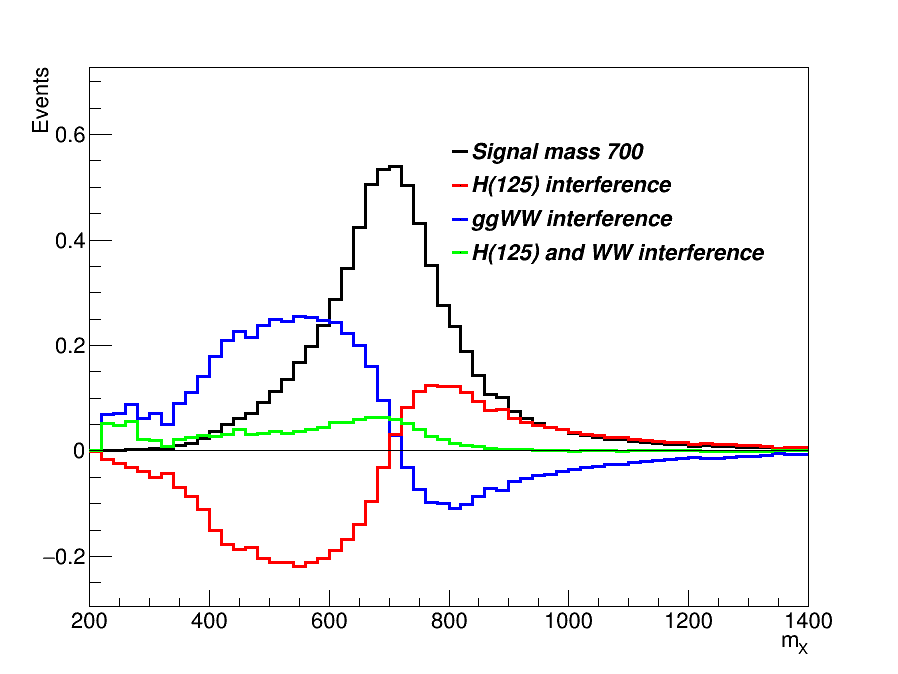
\includegraphics[width=0.45\textwidth]{Figs/Interference_higgsLHEmass700_cuts_nocuts.png}
}
\subfigure[mass 1500 \GeV]{
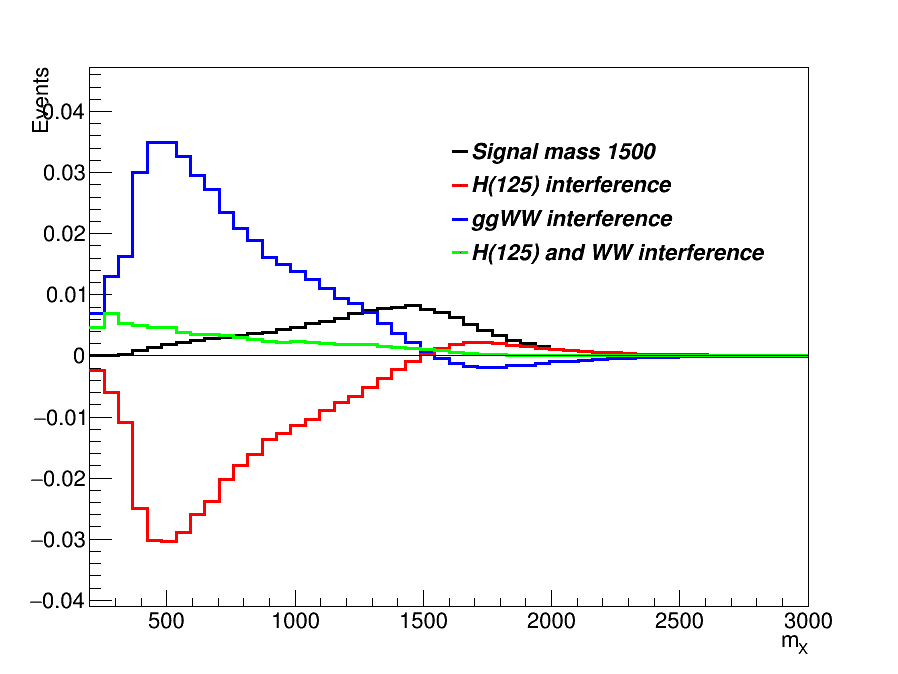
\includegraphics[width=0.45\textwidth]{Figs/Interference_higgsLHEmass1500_cuts_nocuts.png}
}
\caption{  Distribution of  for the X mass resonance at 300-400-700-1500 \GeV.}
    \label{fig:X300}
\end{figure}



\begin{figure}[htb]
\centering
\subfigure[ $m_T^H$ 0 jet]{
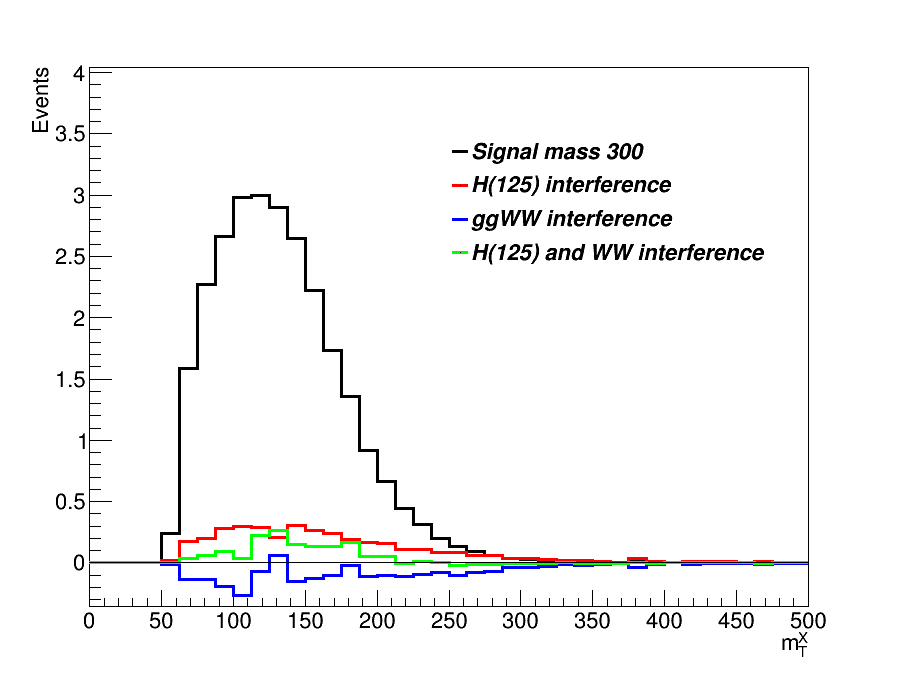
\includegraphics[width=0.35\textwidth]{Figs/Interference_mth300_cuts_0jet.png}
}
\subfigure[$m \ell\ell$ 0 jet]{
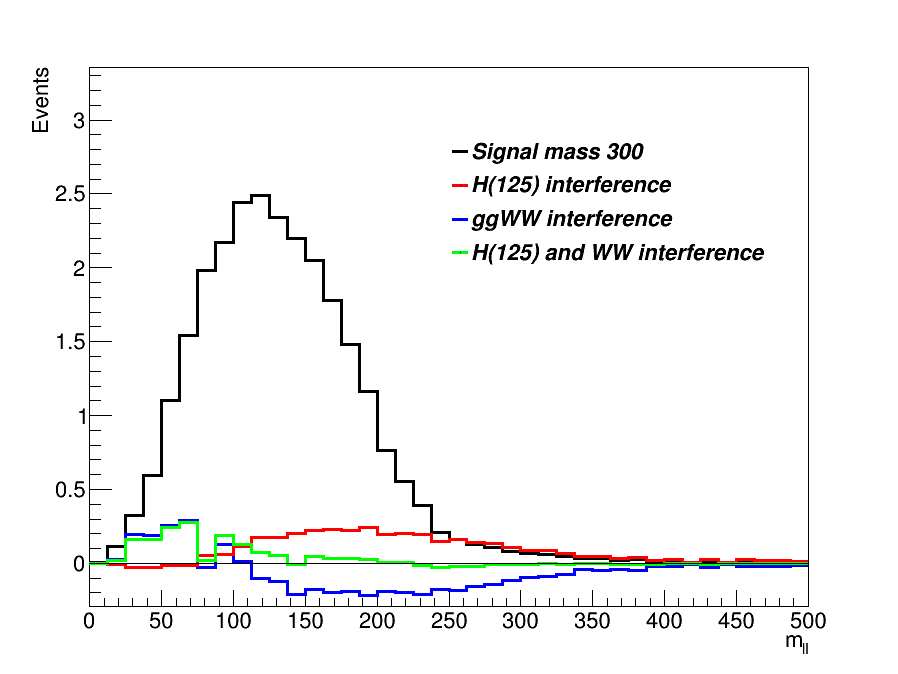
\includegraphics[width=0.35\textwidth]{Figs/Interference_mll300_cuts_0jet.png}
}
\subfigure[$m_T^I$ 0 jet]{
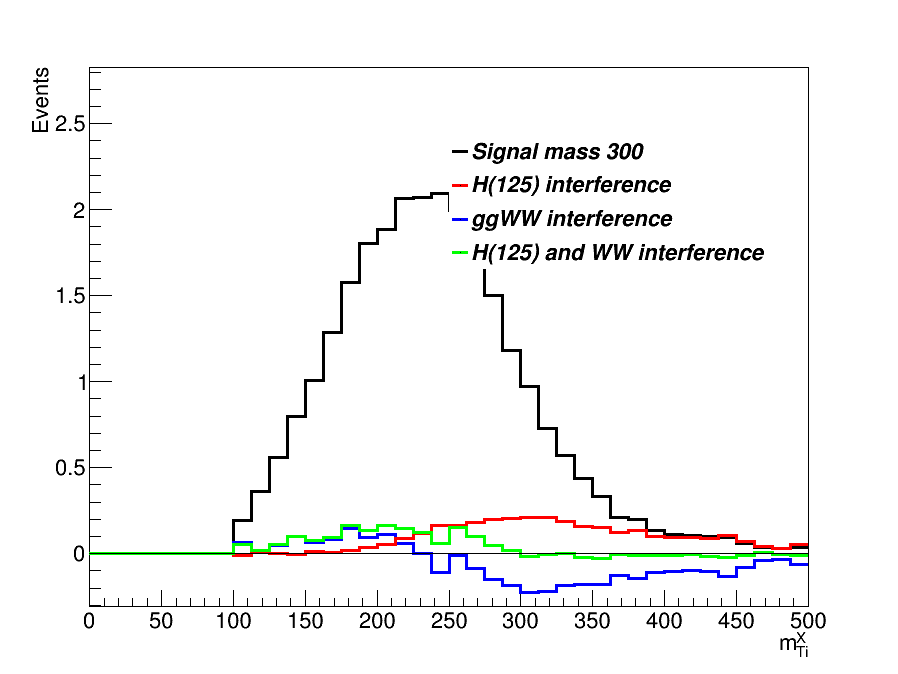
\includegraphics[width=0.35\textwidth]{Figs/Interference_mTi300_cuts_0jet.png}
}\\

\subfigure[ $m_T^H$ 1 jet]{
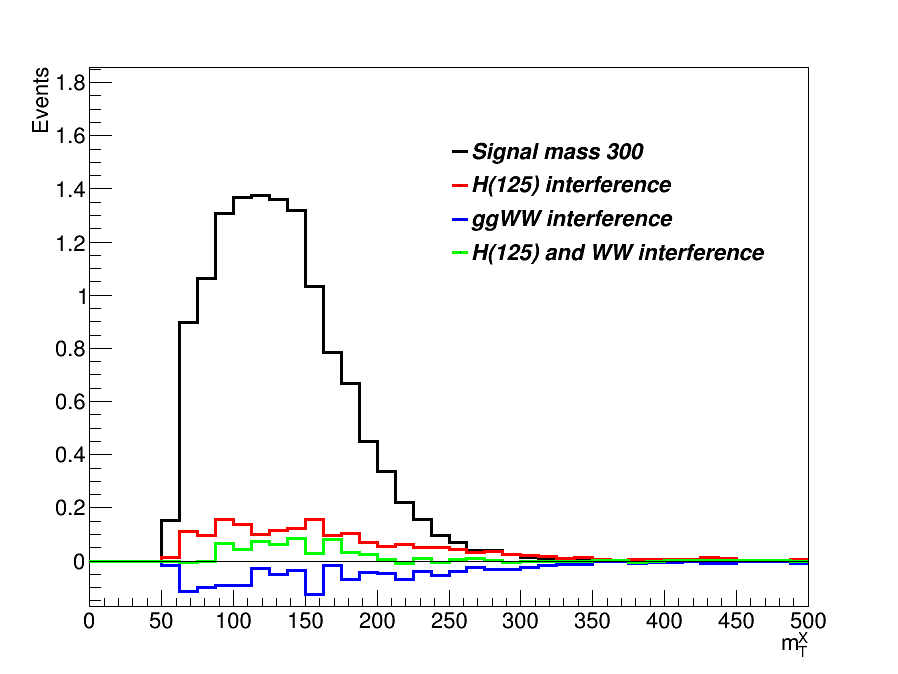
\includegraphics[width=0.35\textwidth]{Figs/Interference_mth300_cuts_1jet.png}
}
\subfigure[$m \ell\ell$ 1 jet]{
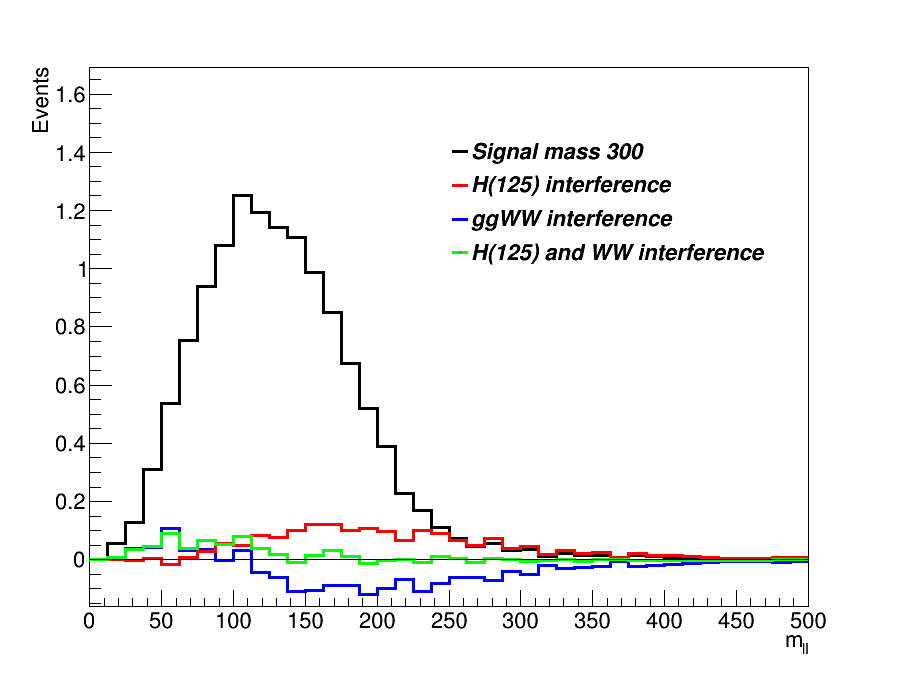
\includegraphics[width=0.35\textwidth]{Figs/Interference_mll300_cuts_1jet.png}
}
\subfigure[$m_T^I$ 1 jet]{
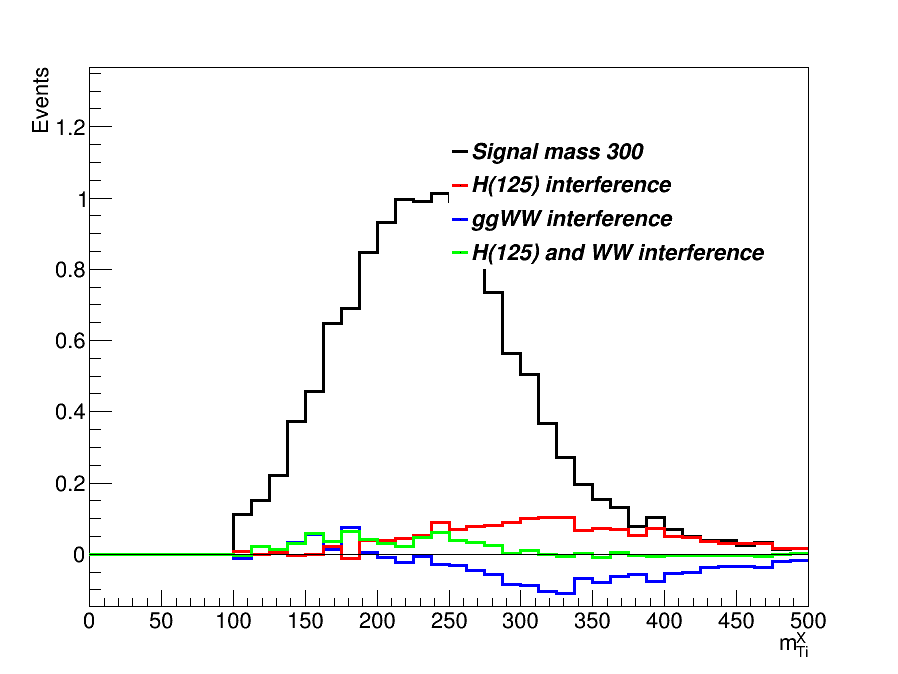
\includegraphics[width=0.35\textwidth]{Figs/Interference_mTi300_cuts_1jet.png}
}\\

\subfigure[ $m_T^H$ 2 jet]{
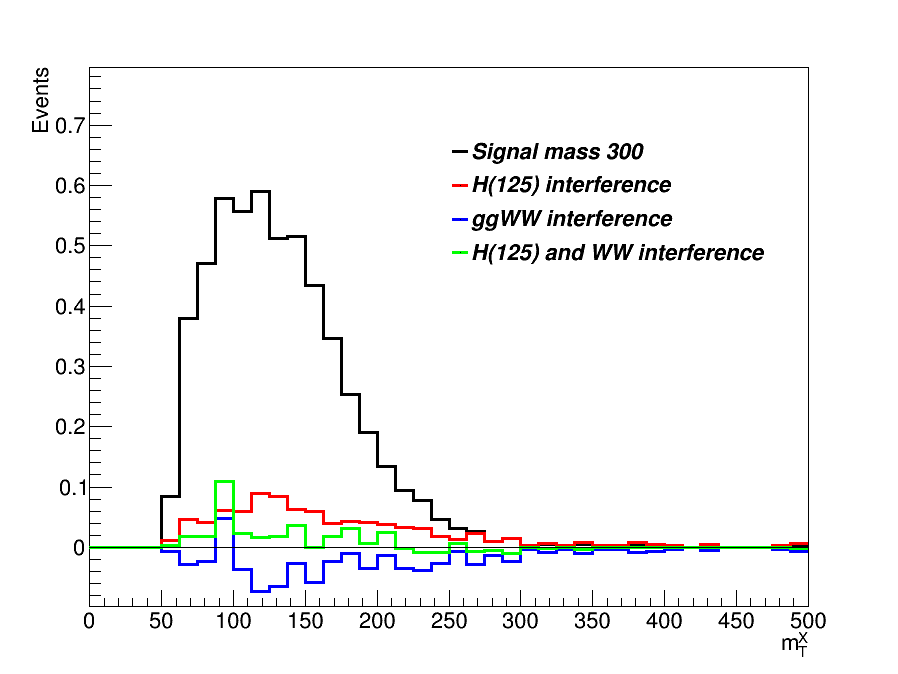
\includegraphics[width=0.35\textwidth]{Figs/Interference_mth300_cuts_2jet.png}
}
\subfigure[$m \ell\ell$ 2 jet]{
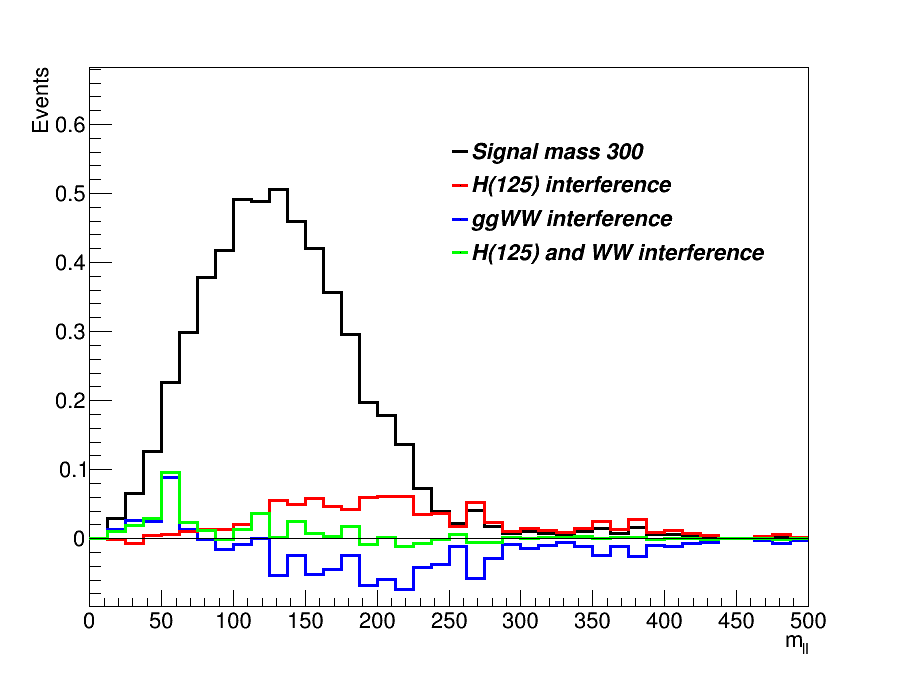
\includegraphics[width=0.35\textwidth]{Figs/Interference_mll300_cuts_2jet.png}
}
\subfigure[$m_T^I$ 2 jet]{
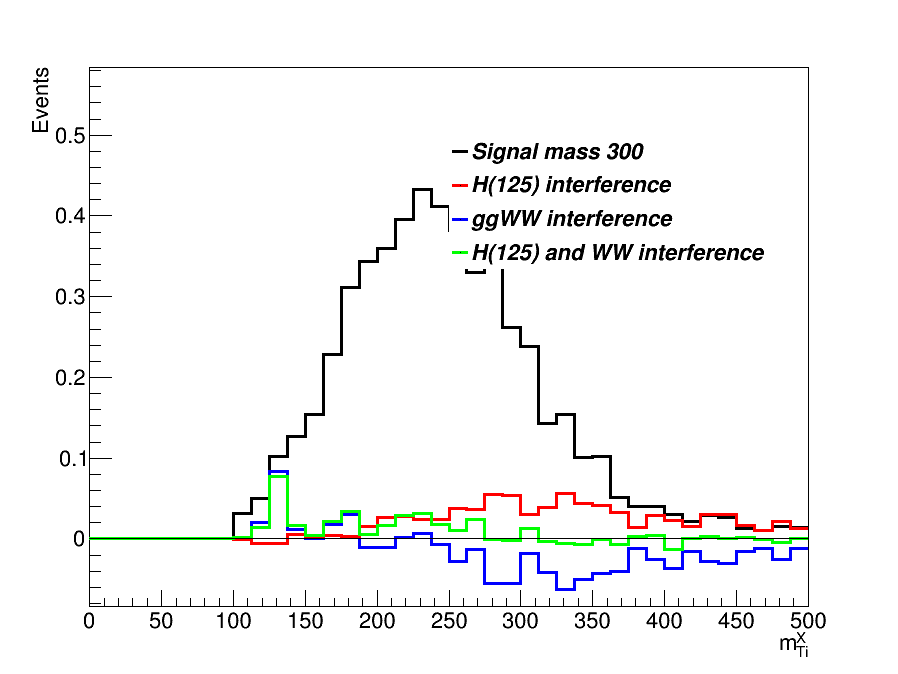
\includegraphics[width=0.35\textwidth]{Figs/Interference_mTi300_cuts_2jet.png}
}\\


\subfigure[ $m_T^H$ VBF]{
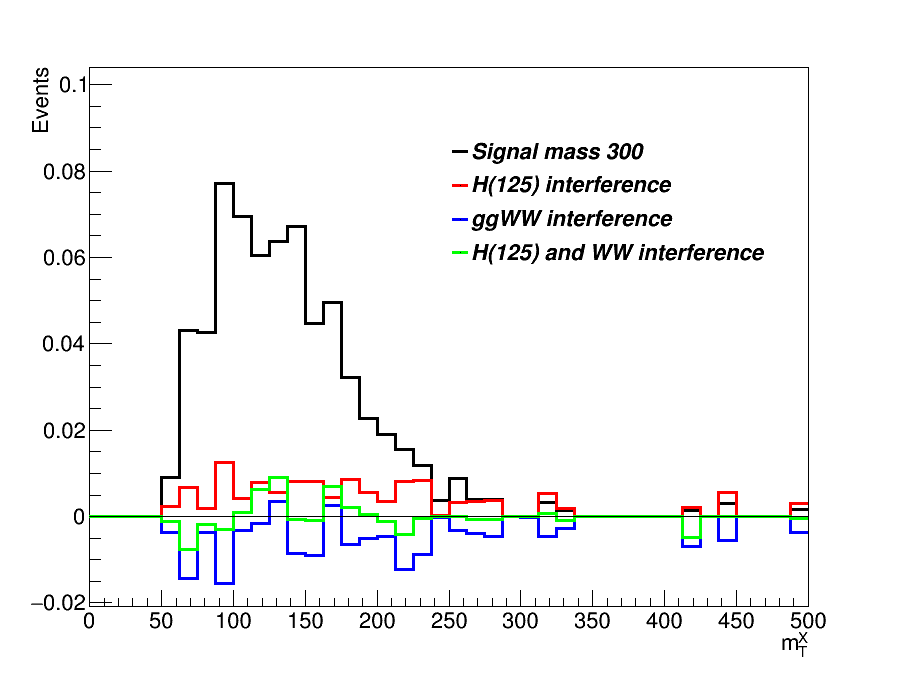
\includegraphics[width=0.35\textwidth]{Figs/Interference_mth300_cuts_VBF2jet.png}
}
\subfigure[$m \ell\ell$ VBF]{
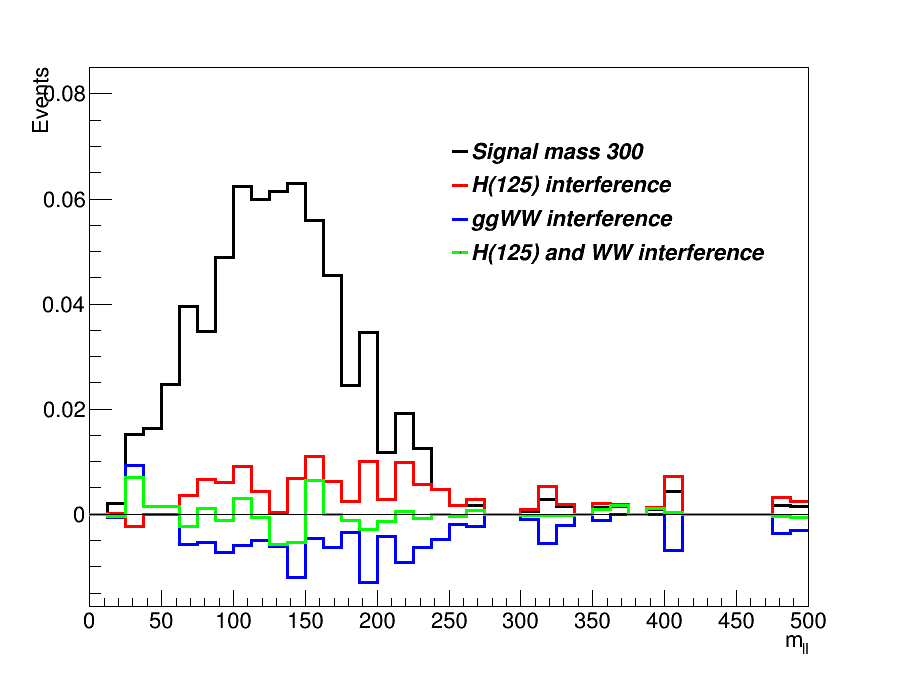
\includegraphics[width=0.35\textwidth]{Figs/Interference_mll300_cuts_VBF2jet.png}
}
\subfigure[$m_T^I$ VBF]{
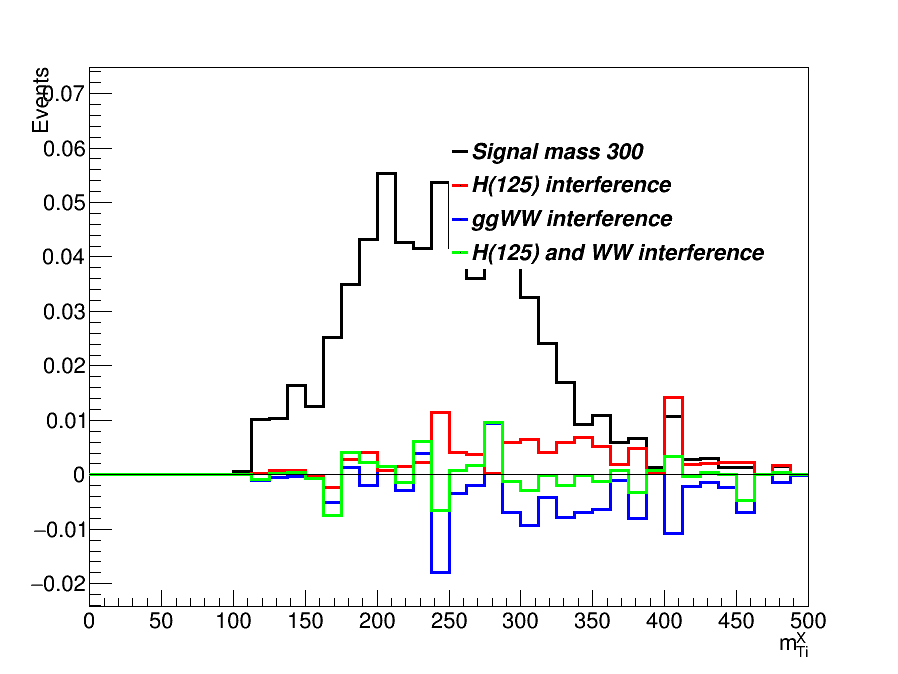
\includegraphics[width=0.35\textwidth]{Figs/Interference_mTi300_cuts_VBF2jet.png}
}\\


\caption{
    Distributions of the  $m_T^H$, $m_{\ell \ell}$ and $m_T^I$ and  variable for sigmal mass of 300\GeV, showing the signal and the interference contribution in the four jet categories.}
    \label{fig:300}
\end{figure}




\begin{figure}[htb]
\centering
\subfigure[ $m_T^H$ 0 jet]{
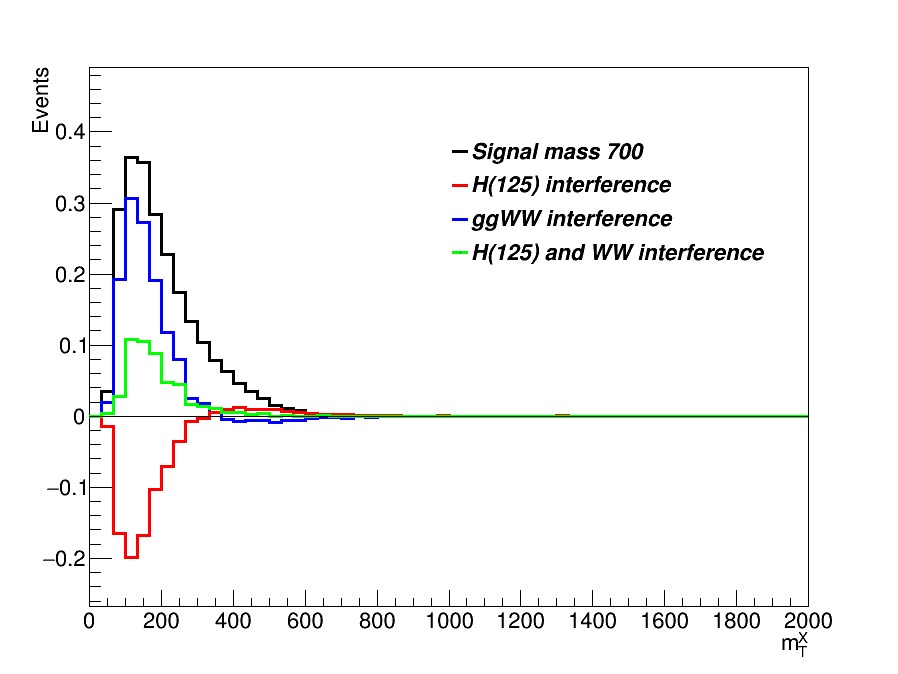
\includegraphics[width=0.35\textwidth]{Figs/Interference_mth700_cuts_0jet.png}
}
\subfigure[$m \ell\ell$ 0 jet]{
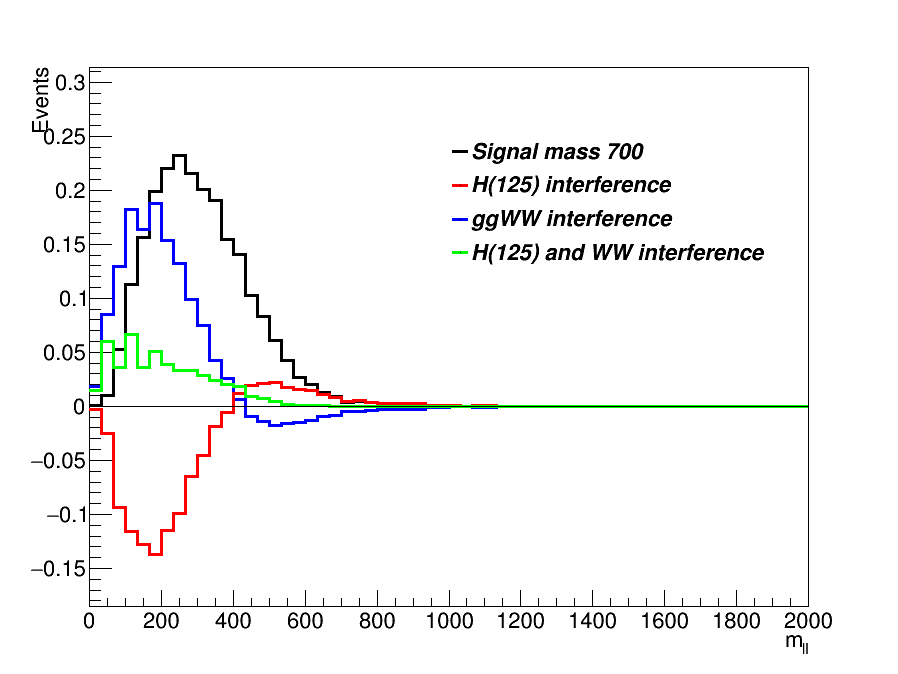
\includegraphics[width=0.35\textwidth]{Figs/Interference_mll700_cuts_0jet.png}
}
\subfigure[$m_T^I$ 0 jet]{
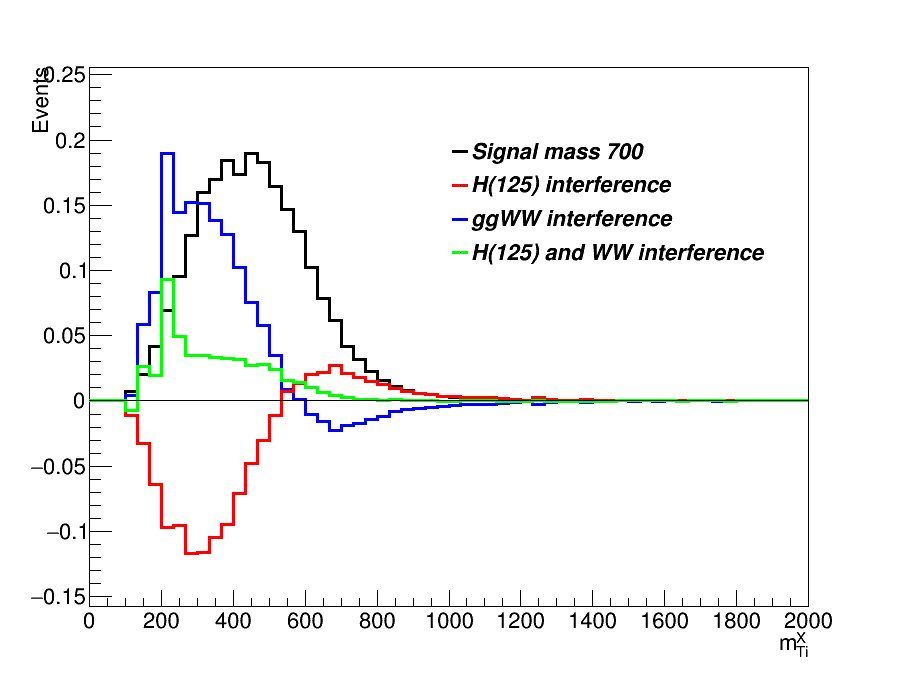
\includegraphics[width=0.35\textwidth]{Figs/Interference_mTi700_cuts_0jet.png}
}\\

\subfigure[ $m_T^H$ 1 jet]{
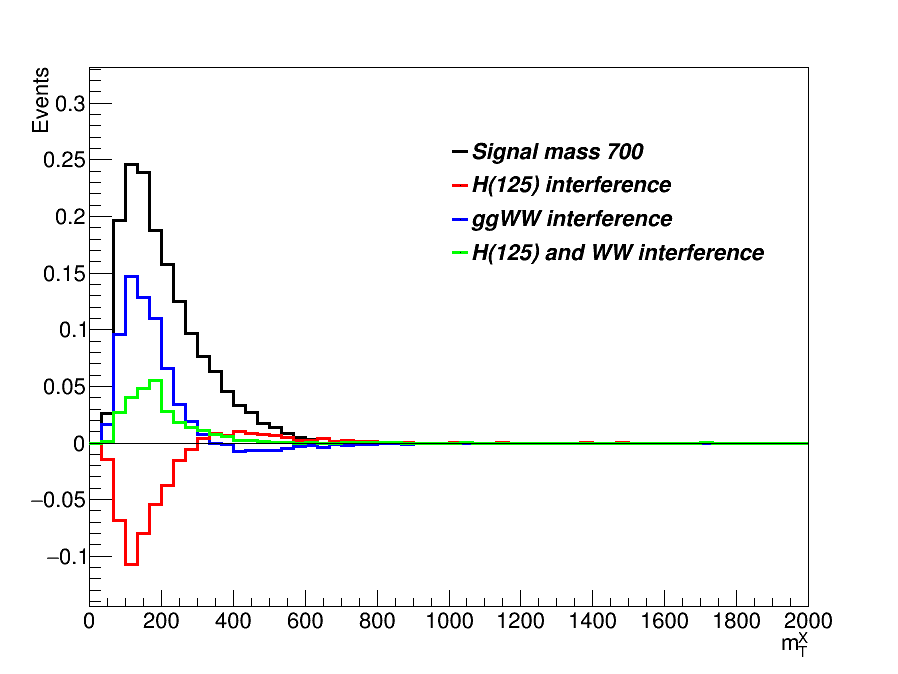
\includegraphics[width=0.35\textwidth]{Figs/Interference_mth700_cuts_1jet.png}
}
\subfigure[$m \ell\ell$ 1 jet]{
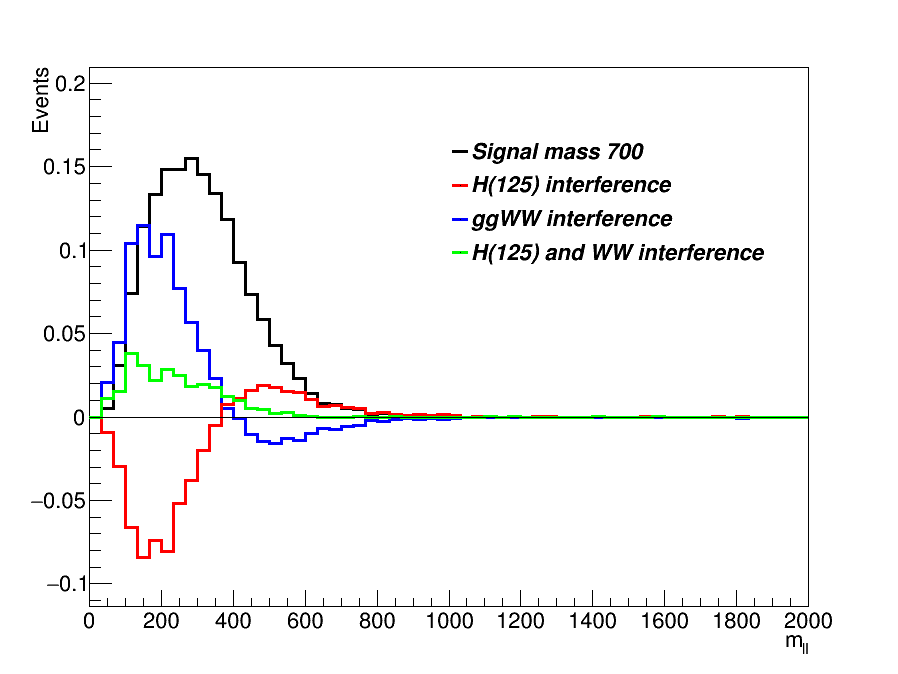
\includegraphics[width=0.35\textwidth]{Figs/Interference_mll700_cuts_1jet.png}
}
\subfigure[$m_T^I$ 1 jet]{
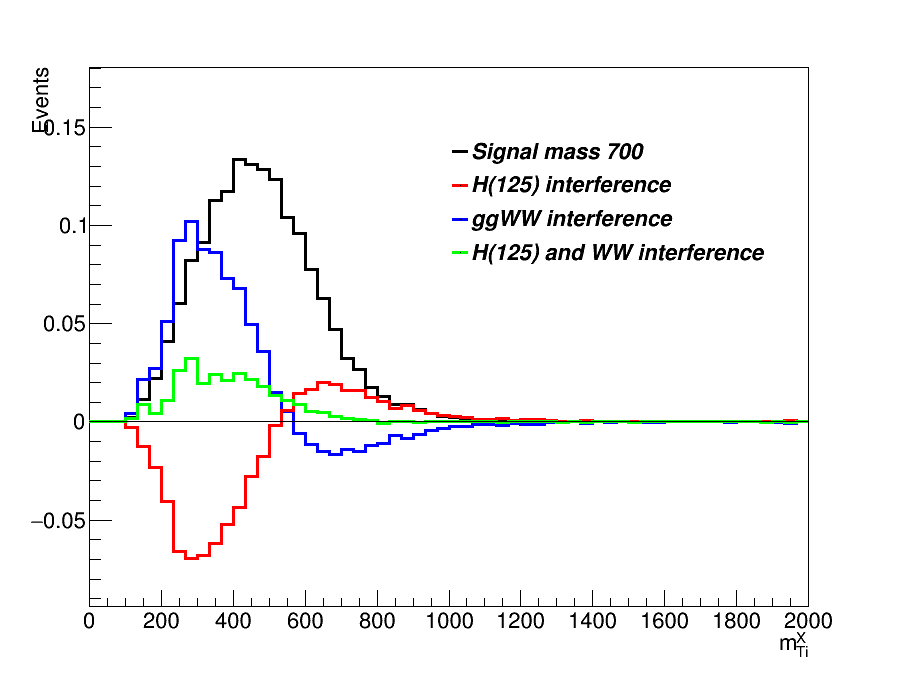
\includegraphics[width=0.35\textwidth]{Figs/Interference_mTi700_cuts_1jet.png}
}\\

\subfigure[ $m_T^H$ 2 jet]{
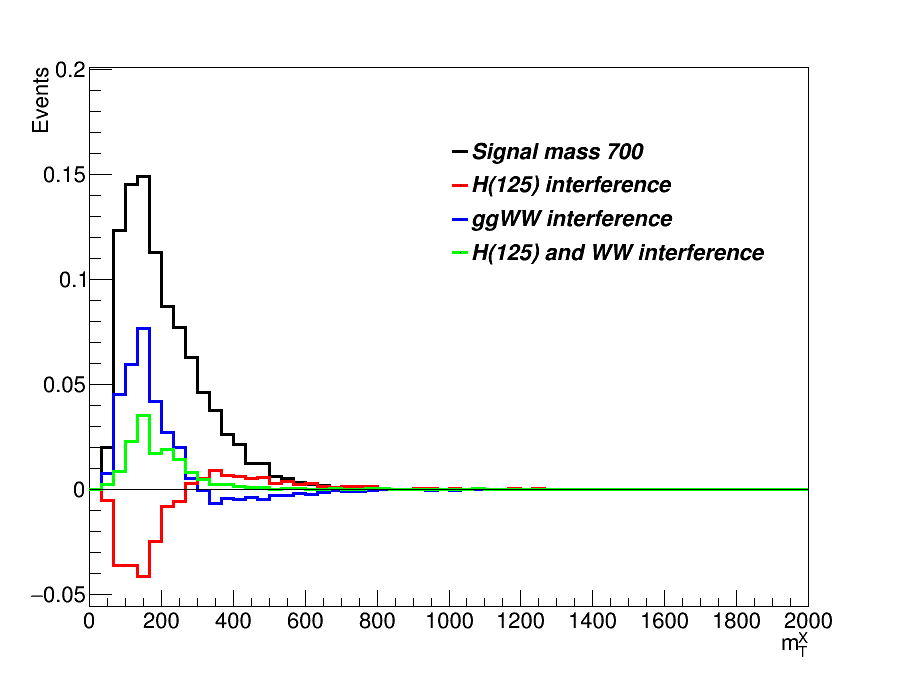
\includegraphics[width=0.35\textwidth]{Figs/Interference_mth700_cuts_2jet.png}
}
\subfigure[$m \ell\ell$ 2 jet]{
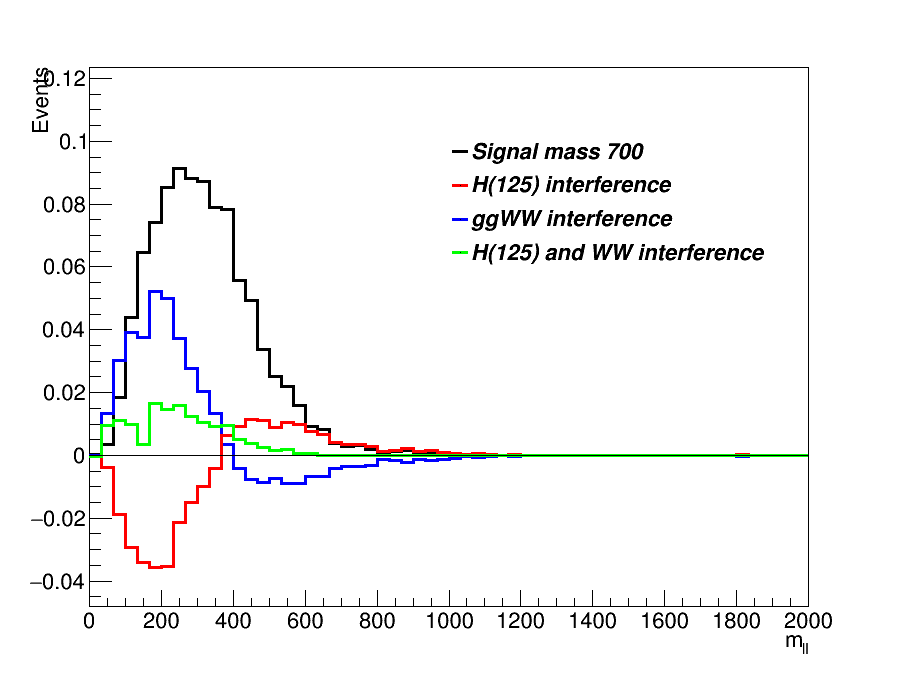
\includegraphics[width=0.35\textwidth]{Figs/Interference_mll700_cuts_2jet.png}
}
\subfigure[$m_T^I$ 2 jet]{
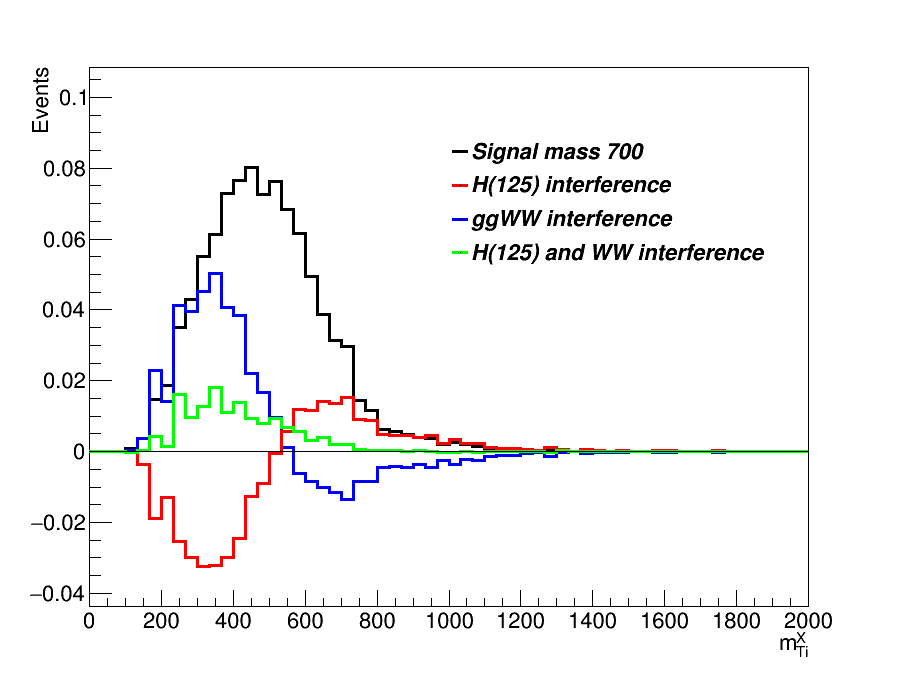
\includegraphics[width=0.35\textwidth]{Figs/Interference_mTi700_cuts_2jet.png}
}\\


\subfigure[ $m_T^H$ VBF]{
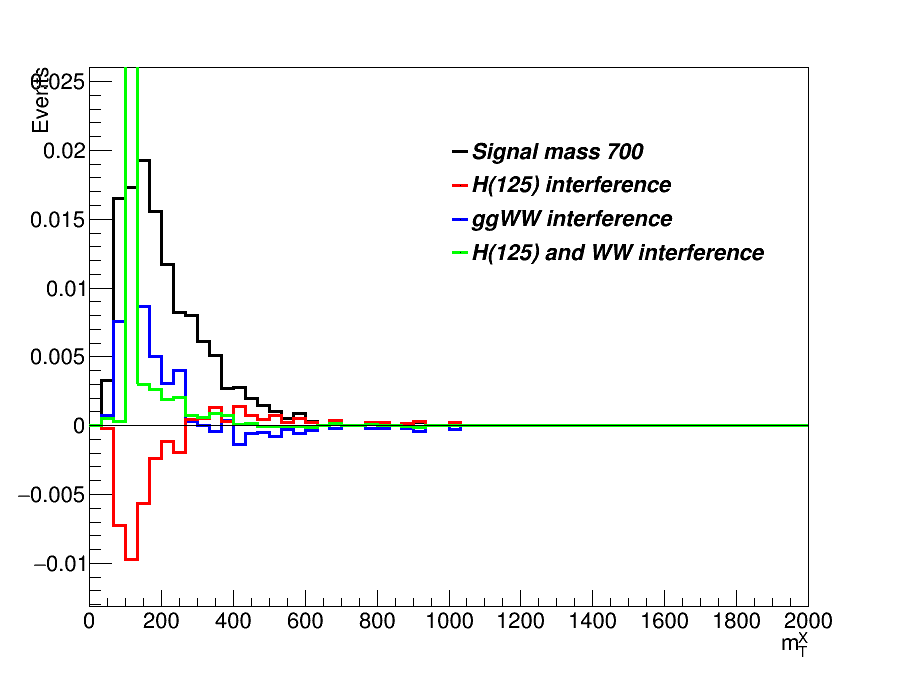
\includegraphics[width=0.35\textwidth]{Figs/Interference_mth700_cuts_VBF2jet.png}
}
\subfigure[$m \ell\ell$ VBF]{
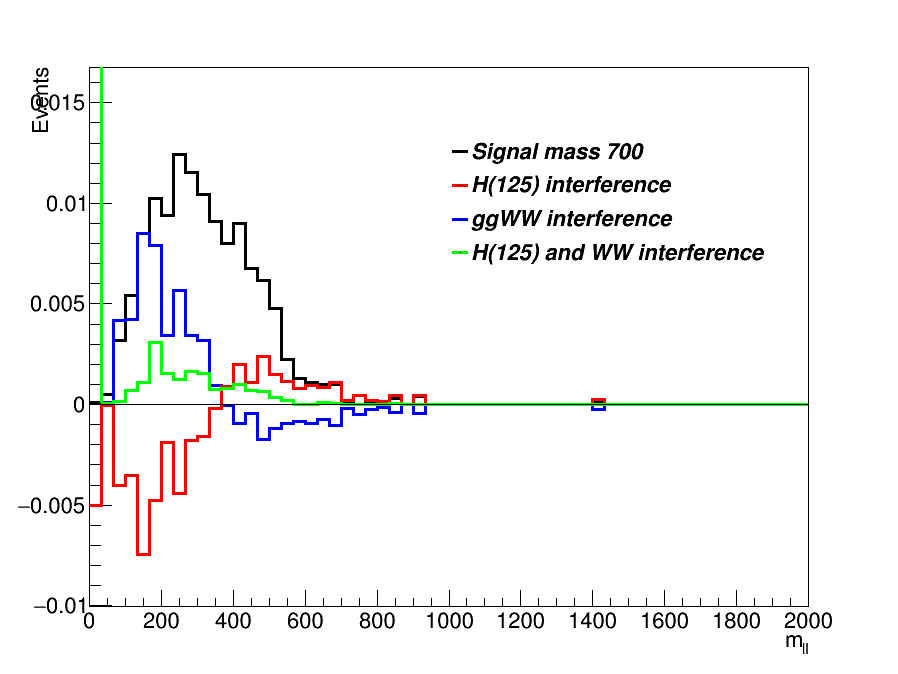
\includegraphics[width=0.35\textwidth]{Figs/Interference_mll700_cuts_VBF2jet.png}
}
\subfigure[$m_T^I$ VBF]{
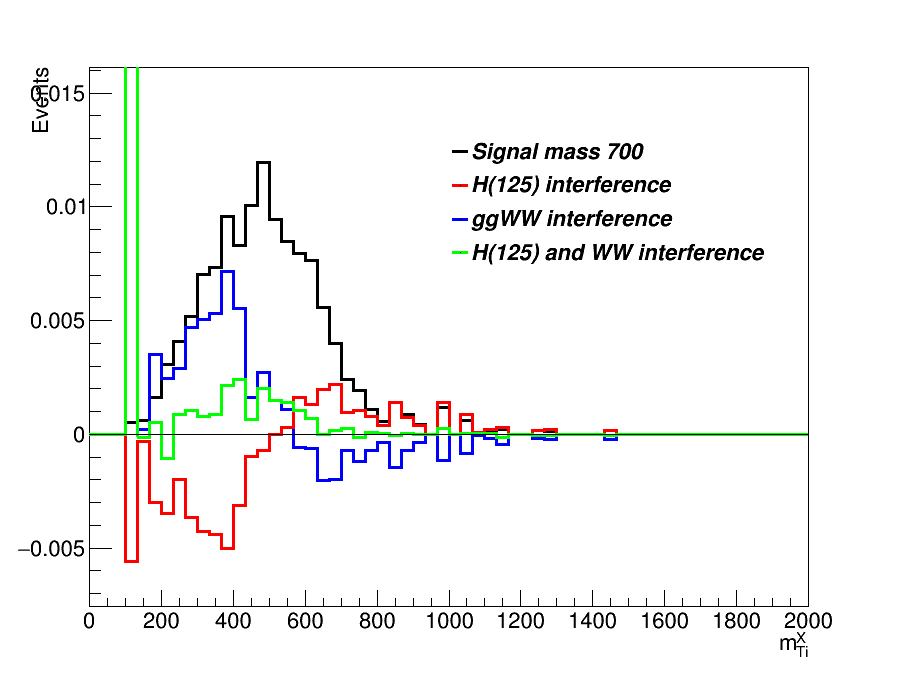
\includegraphics[width=0.35\textwidth]{Figs/Interference_mTi700_cuts_VBF2jet.png}
}\\


\caption{
    Distributions of the  $m_T^H$, $m_{\ell \ell}$ and $m_T^I$ and  variable for sigmal mass of 700\GeV, showing the signal and the interference contribution in the four jet categories.}
    \label{fig:700}
\end{figure}








\begin{figure}[htb]
\centering
\subfigure[ $m_T^H$ 0 jet]{
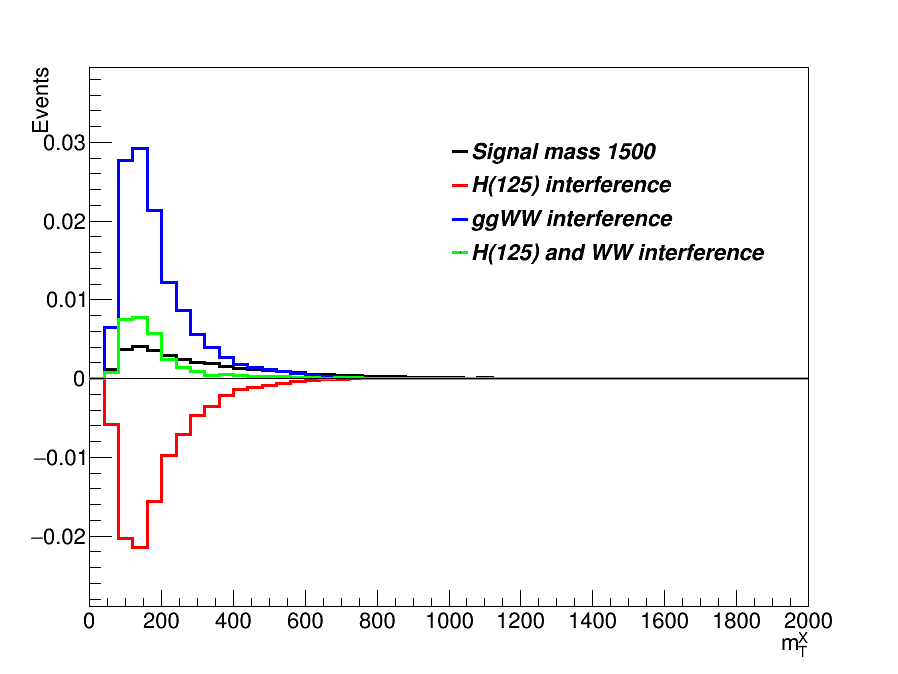
\includegraphics[width=0.35\textwidth]{Figs/Interference_mth1500_cuts_0jet.png}
}
\subfigure[$m \ell\ell$ 0 jet]{
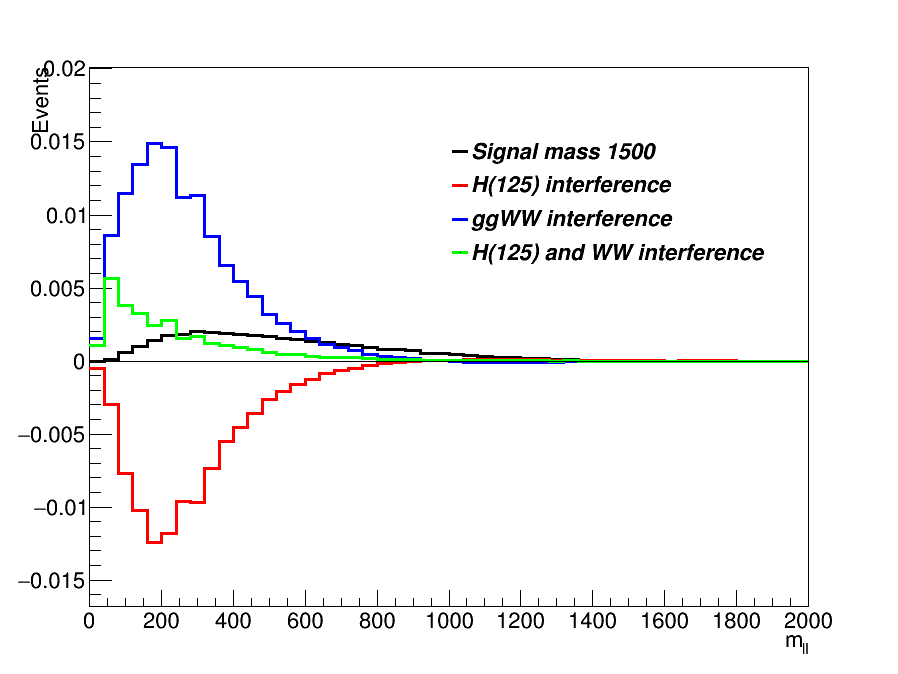
\includegraphics[width=0.35\textwidth]{Figs/Interference_mll1500_cuts_0jet.png}
}
\subfigure[$m_T^I$ 0 jet]{
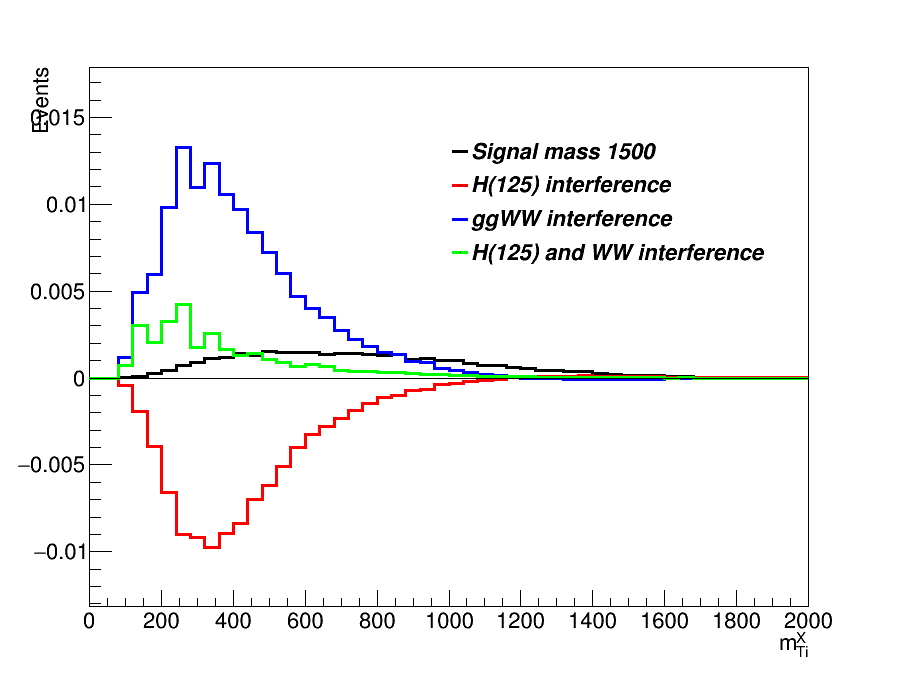
\includegraphics[width=0.35\textwidth]{Figs/Interference_mTi1500_cuts_0jet.png}
}\\

\subfigure[ $m_T^H$ 1 jet]{
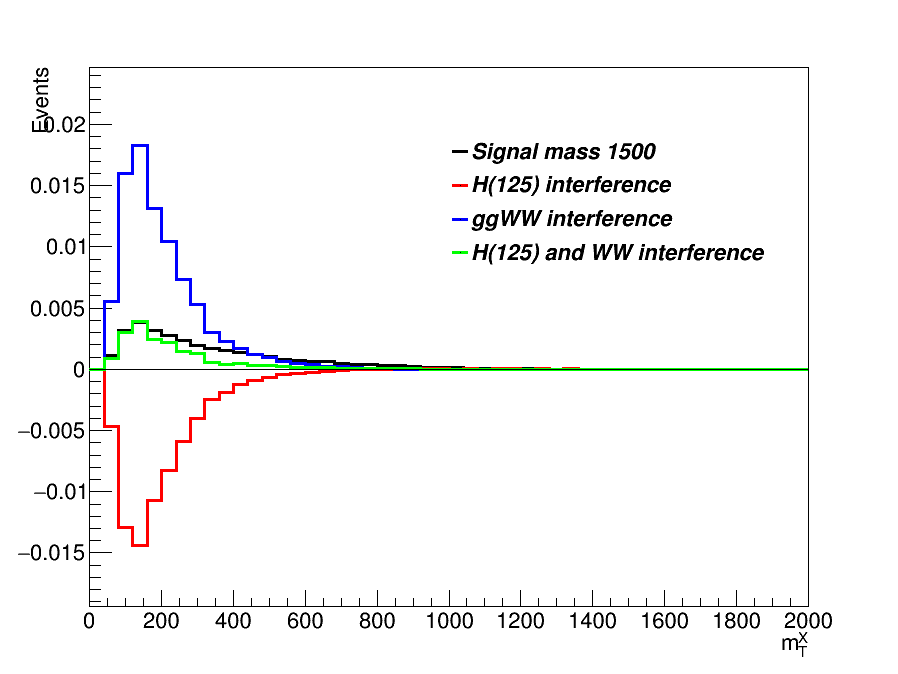
\includegraphics[width=0.35\textwidth]{Figs/Interference_mth1500_cuts_1jet.png}
}
\subfigure[$m \ell\ell$ 1 jet]{
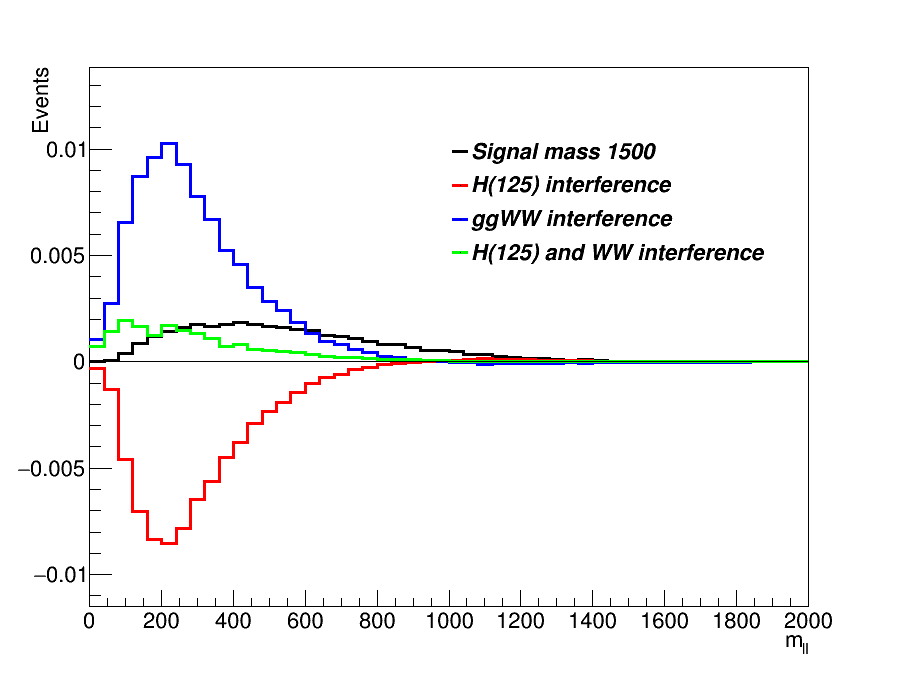
\includegraphics[width=0.35\textwidth]{Figs/Interference_mll1500_cuts_1jet.png}
}
\subfigure[$m_T^I$ 1 jet]{
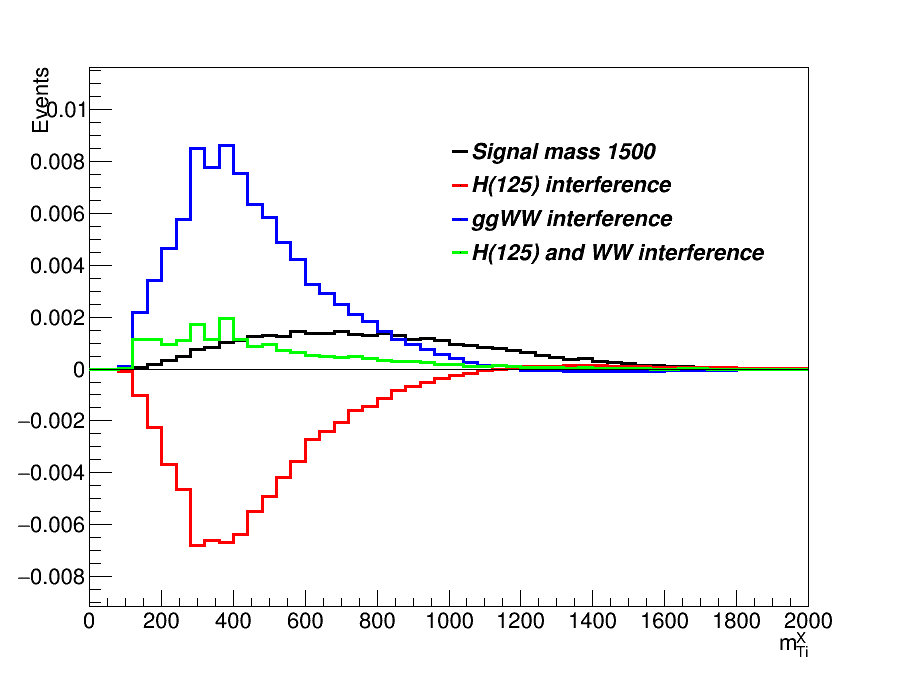
\includegraphics[width=0.35\textwidth]{Figs/Interference_mTi1500_cuts_1jet.png}
}\\

\subfigure[ $m_T^H$ 2 jet]{
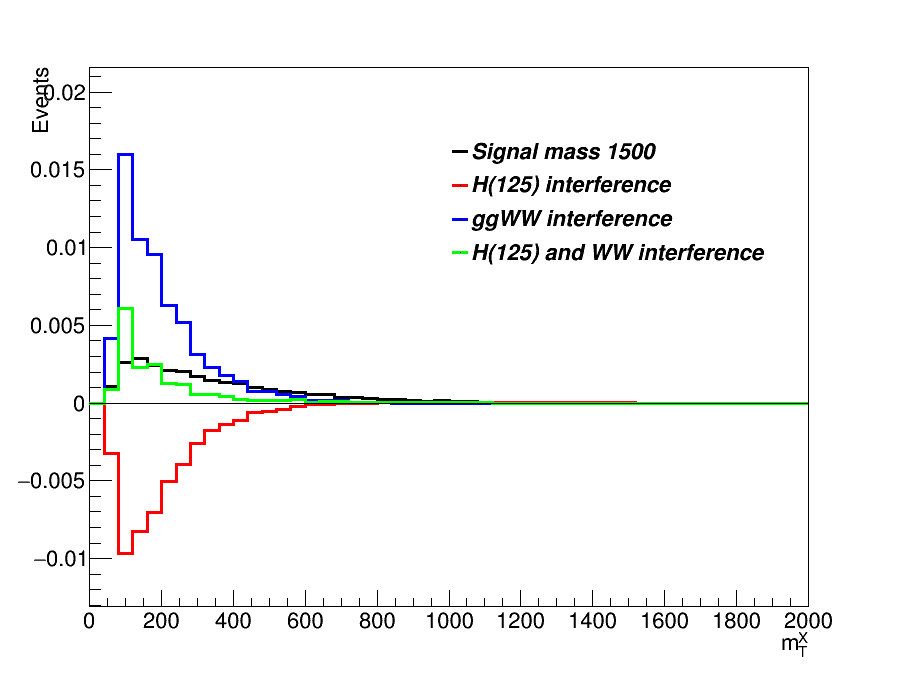
\includegraphics[width=0.35\textwidth]{Figs/Interference_mth1500_cuts_2jet.png}
}
\subfigure[$m \ell\ell$ 2 jet]{
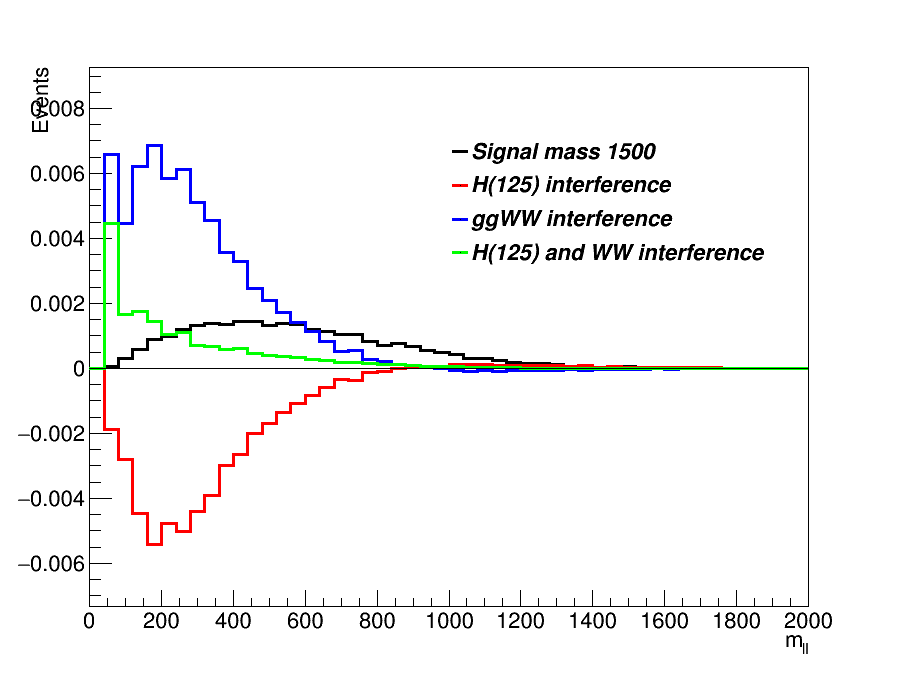
\includegraphics[width=0.35\textwidth]{Figs/Interference_mll1500_cuts_2jet.png}
}
\subfigure[$m_T^I$ 2 jet]{
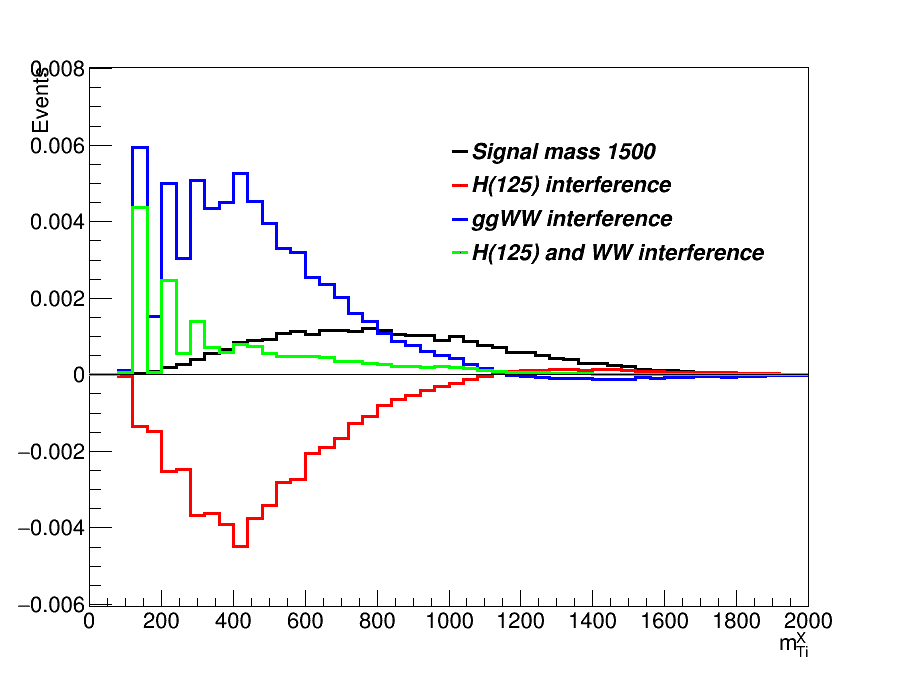
\includegraphics[width=0.35\textwidth]{Figs/Interference_mTi1500_cuts_2jet.png}
}\\


\subfigure[ $m_T^H$ VBF]{
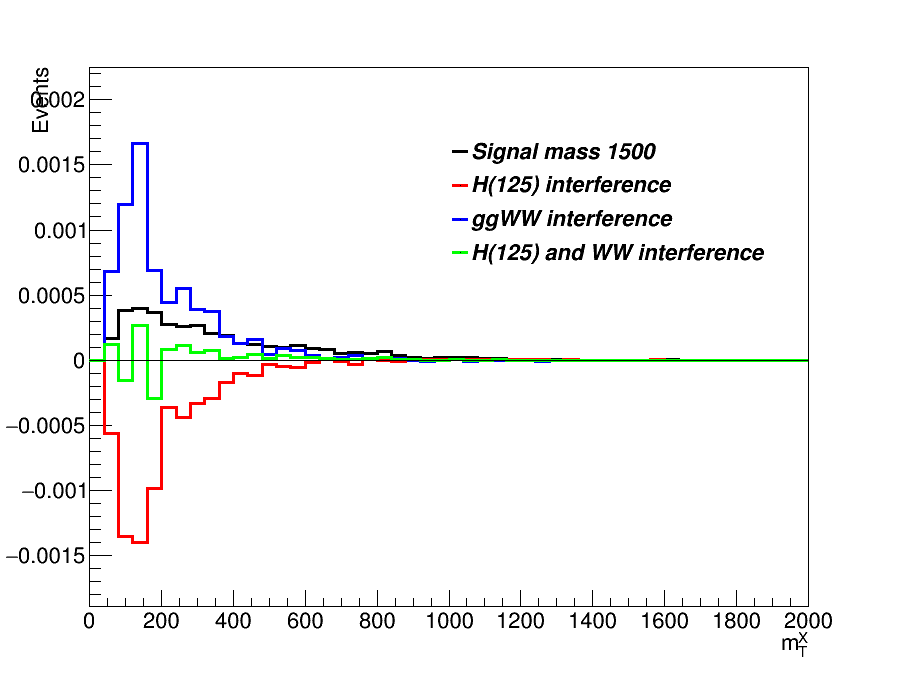
\includegraphics[width=0.35\textwidth]{Figs/Interference_mth1500_cuts_VBF2jet.png}
}
\subfigure[$m \ell\ell$ VBF]{
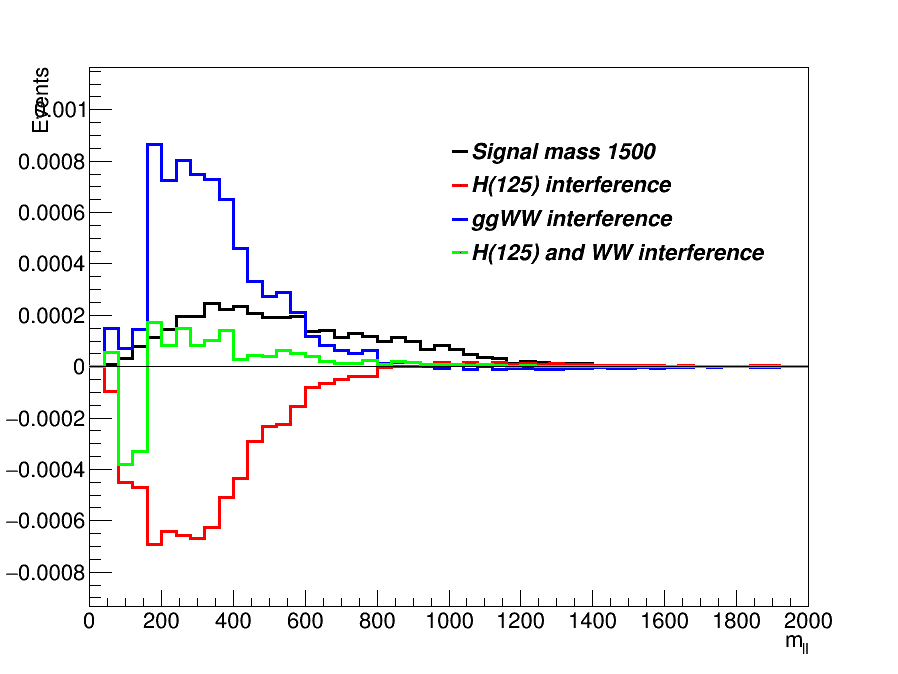
\includegraphics[width=0.35\textwidth]{Figs/Interference_mll1500_cuts_VBF2jet.png}
}
\subfigure[$m_T^I$ VBF]{
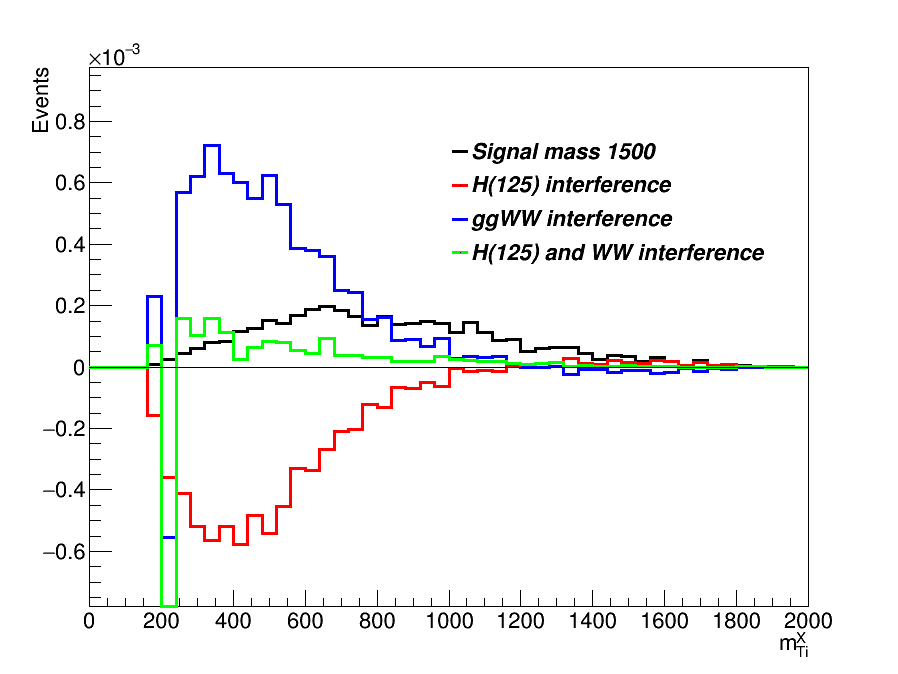
\includegraphics[width=0.35\textwidth]{Figs/Interference_mTi1500_cuts_VBF2jet.png}
}\\


\caption{
    Distributions of the  $m_T^H$, $m_{\ell \ell}$ and $m_T^I$ and  variable for sigmal mass of 1500\GeV, showing the signal and the interference contribution in the four jet categories.}
    \label{fig:1500}
\end{figure}






\subsection{Study of the interference effects: VBF case}
\label{sec:interference_VBF}
The interference is also evaluate for the VBF signal mechanism production. In this case the interference occurs between 
